% This file is iccc.tex.  It contains the formatting instructions for and acts as a template for submissions to ICCC.  It borrows liberally from the AAAI and IJCAI formats and instructions.  It uses the files iccc.sty, iccc.bst and iccc.bib, the first two of which also borrow liberally from the same sources.


\documentclass[letterpaper]{article}
\usepackage{iccc}

\usepackage{graphicx}       % figures
\usepackage{float}

\usepackage{times}
\usepackage{helvet}
\usepackage{courier}
\pdfinfo{
/Title (SpaceSheet: Navigating Conceptual Space with a Spreadsheet Interface)
/Subject (Proceedings of ICCC)
/Author (ICCC)}
% The file iccc.sty is the style file for ICCC proceedings.
%
\title{SpaceSheet: Navigating Conceptual Space with a Spreadsheet Interface}
\author{
  Tom White and Bryan Loh\\
  School of Design\\University of Wellington\\Wellington, New Zealand \\
  \texttt{\{tom.white@vuw.ac.nz, lohbrya@myvuw.ac.nz\}} \\
}
\setcounter{secnumdepth}{0}

\begin{document} 
\maketitle
\begin{abstract}
\begin{quote}
We introduce a new spreadsheet based interface called SpaceSheets for creating novel images and other media. Unlike traditional digital tools, ours is parameterized entirely by a neural network with no preprogrammed rules or knowledge representations. The capability of SpaceSheets to support visual exploration and communication is demonstrated within the context of several domains including facial images, fonts, and english words. SpaceSheets is demonstrated to support the experimentation and exploration of latent spaces enabling more effective design experimentation.
\end{quote}
\end{abstract}

\section{Introduction}

Problem solving can be viewed as a search for a solution within a space. In design, this process involves generating solutions and evaluating their consequences relative to goals and constraints~\cite{simon95}. These experiments are enabled through representations in the form of drawings and diagrams. Computational design tools enable users to construct and manipulate representations digitally. These tools often impose a high cost to design experimentation due to the mismatch between low-level design operations in expressing more abstract design intent.

Generative models learn more compact representations of the training data in a vector space of latent variables. Latent variables are sampled from high-dimensional latent space and can be decoded back into observable values. Additionally, semantic operations can be performed within latent space using vector arithmetic~\cite{white16}.

Spreadsheet interfaces are a ubiquitous part of office productivity suites. They enable users to perform experimental calculations using a set of formulae which define relationships spatially. Automatic recalculation supports experimentation by enabling users to observe the results of their actions immediately and act accordingly.

\begin{figure}[ht]
  \centering
  % \fbox{\rule[-.5cm]{0cm}{4cm} \rule[-.5cm]{4cm}{0cm}}
  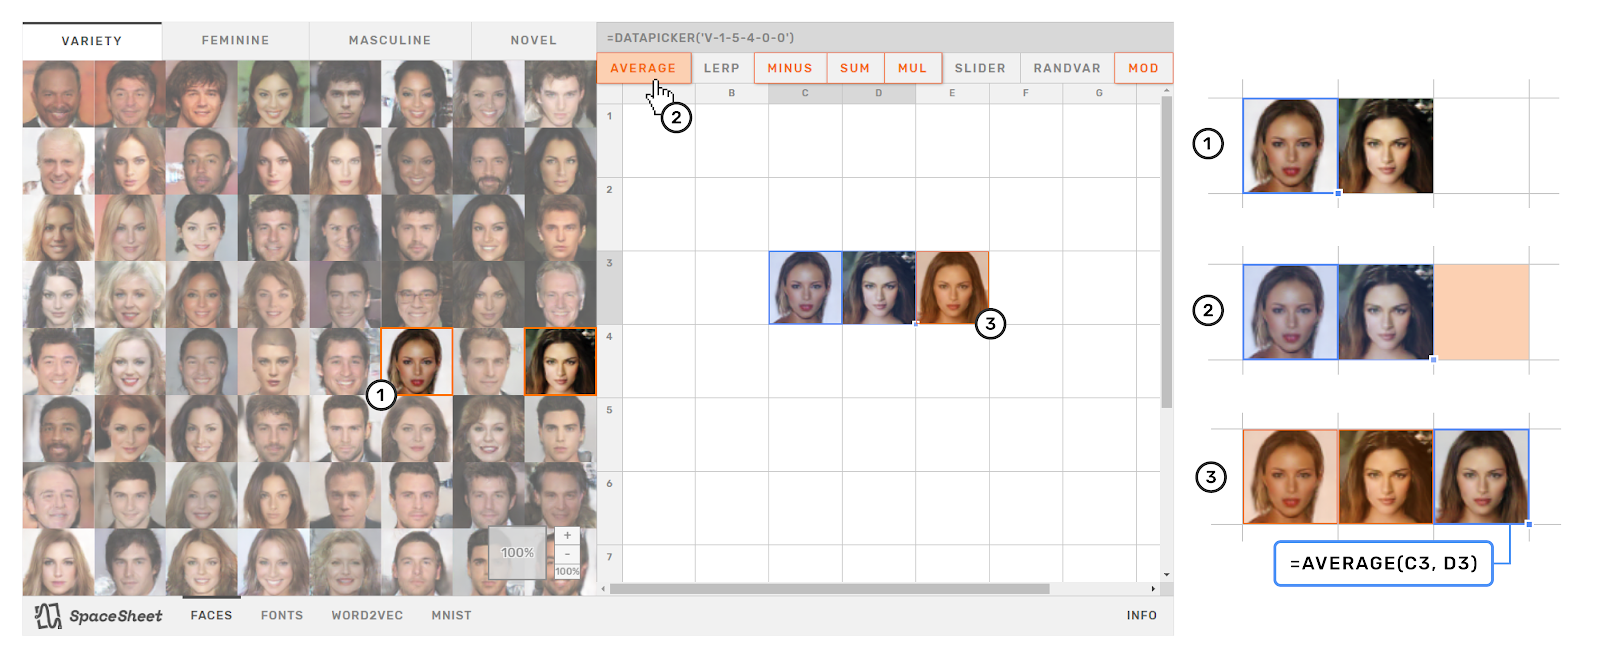
\includegraphics[width=8cm]{figs/01-hero-diagram.png}
  \caption{The SpaceSheet being used to perform an average between two latent variables}
\end{figure}

We developed SpaceSheet (Figure 1) to leverage the familiarity and power of spreadsheet interfaces for the purpose of design experimentation within latent space. It has been adapted to enable non-experts to explore and experiment within latent spaces.

\section{Background}

\subsection{Conceptual Spaces}

Generative models are a popular approach to unsupervised machine learning. Generative neural network models are trained to produce data samples that resemble the training set ~\cite{openai1}. Because the number of model parameters is significantly smaller than the training data, the models are forced to discover efficient data representations. These models are sampled from a set of latent variables in a high-dimensional space, called a latent space. Latent space can be sampled to generate observable data values. Learned latent representations often also allow semantic operations with vector space arithmetic (Figure 2), a phenomenon discovered previously in the latent space of language models~\cite{word2vec}.

\begin{figure}[ht]
  \centering
  % \fbox{\rule[-.5cm]{0cm}{4cm} \rule[-.5cm]{4cm}{0cm}}
  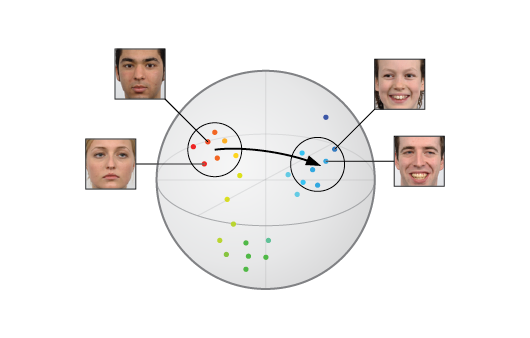
\includegraphics[width=8cm]{figs/face_space.png}
  \caption{Schematic of the latent space of a generative model. In the general case, a generative model includes an encoder to map from the feature space (here images of faces) into a high-dimensional latent space. Vector space arithmetic can be used in the latent space to perform semantic operations. The model also includes a decoder to map from the latent space back into the feature space, where the semantic operations can be observed. If the latent space transformation is the identity function we refer to the encoding and decoding as a reconstruction of the input through the model. }
\end{figure}

Generative models are often applied to datasets of images. Two popular generative models for image data are the Variational Autoencoder~\cite{kingma13} (VAE) and the Generative Adversarial Network~\cite{goodfellow14} (GAN). VAEs use the framework of probabilistic graphical models with an objective of maximizing a lower bound on the likelihood of the data. GANs instead formalize the training process as a competition between a generative network and a separate discriminative network. Though these two frameworks are very different, both construct high-dimensional latent spaces that can be sampled to generate images resembling training set data. Moreover, these latent spaces are generally highly structured and can enable complex operations on the generated images by simple vector space arithmetic in the latent space~\cite{larsen15}.

In the latent space of generative models, many high-level attributes can be represented as a vector (Figure 3). Using techniques from ~\cite{white16}, multiple attributes can be decoupled further to create a visualization of possible states across multiple semantic vectors (Figure 4). For example, when trained on a dataset of portraits, latent vectors can be computed for "smiling" and "mouth open" which then applied to new face images.

\begin{figure}[ht]
  \centering
  % \fbox{\rule[-.5cm]{0cm}{4cm} \rule[-.5cm]{4cm}{0cm}}
  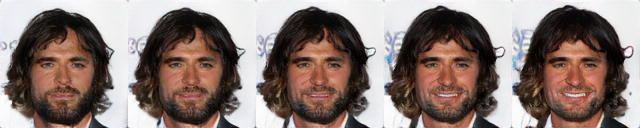
\includegraphics[width=8cm]{figs/smilevector.png}
  \caption{Traversals along the smile vector using a GAN model from ~\cite{dumoulin16}}
\end{figure}

\begin{figure}[ht]
  \centering
  % \fbox{\rule[-.5cm]{0cm}{4cm} \rule[-.5cm]{4cm}{0cm}}
  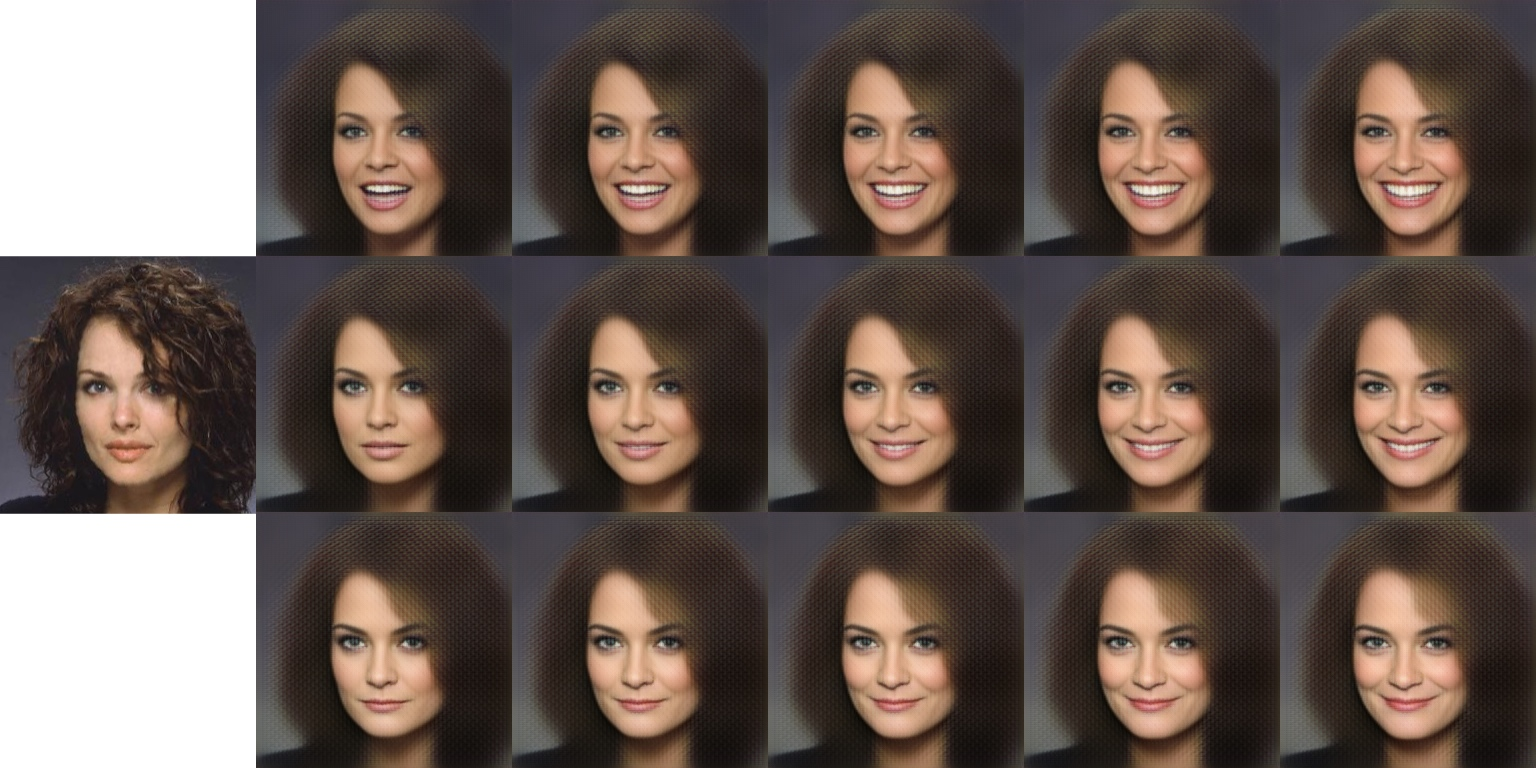
\includegraphics[width=8cm]{figs/decoupled.jpg}
  \caption{Decoupling attribute vectors for smiling (x-axis) and mouth open (y-axis) allows for more flexible latent space transformations. Input shown at left with reconstruction adjacent. Using a VAE model from ~\cite{lamb16}}
\end{figure}

Prior to the discovery of neural network latent spaces supporting semantic operations, cognitive science had hypothesized the existence of knowledge representations that were primarily geometric instead of symbolic. One primary proponent was G{\"{a}}rdenfors who proposed a framework of "Conceptual Spaces" as structured multi-dimensional feature spaces to support modeling information processes such as concept learning and prototype theory~\cite{gardenfors11}. Notably, conceptual spaces were proposed as a model of how people structure concepts, independent of any proposed computational implementation of how they might come about.

We adapt the terminology and claim that latent spaces of generative neural networks function as conceptual spaces which can be used as non-symbolic knowledge representation layers in other tools. With this framework, we examine the ability of this representation layer built from the latent space of a generative neural network model to support a new type of spreadsheet interface tool. The tool itself is domain independent and is shown to be useful in several domains. In exploring these particular domains, our tool constructs subspaces of the larger conceptual space of possibilities as a parameter space of a spreadsheet driven exploration tool.

\subsection{Supporting Design Experimentation}

Design principles have been identified by ~\cite{resnick05} and ~\cite{terry02}
for user interfaces to support design experimentation and exploration.

These principles can be summarised by the three user interface requirements proposed in Design Principles for Tools to Support Creative Thinking~\cite{resnick05}  (paraphrased):
It must be very easy to try things out and then backtrack when unsuccessful.
Tools should be ‘self-revealing’ in what they can achieve.
Make it very fast to sketch out different alternatives

These principles are supported by ~\cite{terry02} where they identify three activities in the process of reflection-in-action~\cite{schon84} that should be supported by user interfaces for design experimentation. They are: Near-Term Experimentation, Generating Variations, and Evaluation.

Near-Term Experimentation is used to describe actions which intend to ``discover and instantiate the next move'' ~\cite[p. 39]{terry02}. In a user interface, users would make hypotheses about the next action to be made, and test their hypothesis by ``invoking a command and adjusting its settings to achieve the imagined effect''. The users would then ``either accept the command, tweak the parameters more, or undo it and try another tact'' ~\cite[p. 40]{terry02}.

Variations are created by the designer to explore alternatives deeply. It enables them ``to better understand the problem, its boundaries, and potential solutions'' ~\cite[p. 40]{terry02}. An example of this is where designers make ``multiple variations of a specific component by creating them side-by-side on a large canvas ... and iterate on promising versions to arrive at an acceptable solution'' ~\cite[p. 40]{terry02}.

Users need to evaluate their progress as they work on a task. This happens after near-term experiments, as well as after generating variations: ``the moment in which the individual reassesses the problem and their understanding of it, before making the next move'' ~\cite[p. 40]{terry02}.

\subsection{Spreadsheet as a Design tool}

Spreadsheets may seem like an unlikely design tool. However, the ability to express relationships between cells make it functionally suited to express operations in latent space. 
Additionally, it satisfies the three user requirements for software to support design experimentation — Near-Term Experimentation, Generating Variations, and Evaluation as proposed by ~\cite{terry02}.

Near-term experimentation is supported by the automatic updating feature of the spreadsheet. Users are able to set up scenarios of logic and calculate the results to ‘what if’ questions instantly by modifying the cell values. This establishes a tight feedback loop between the user’s actions and its implications. When coupled with the ability to undo actions, it enables users to discover and instantiate moves, and backtrack if the results are unsatisfactory.

The generation of variations is supported by enabling users to duplicate instances of data onto other cells within the document. These copies can then be modified independently from the original data.

Evaluation is supported by enabling users flexibility in how they choose to organise data in the document. Users can set up custom templates in a layout which best supports their preferences and the problem to be solved.

In addition to their promise in supporting design experimentation, spreadsheet software is well-established within office productivity suites. Users with an understanding of how conventional spreadsheets function are able to transfer their understanding to the use of the design tool.

\section{SpaceSheet}

SpaceSheet consists of a data picker exposing latent variables to operate with and a spreadsheet to define operations between the variables. In both, latent variables are decoded into observable images.

\subsection{Data Picker}

The data picker is a predetermined set of latent variables which have been organized into a grid. The set of variables in the data picker act as the points of reference from which the latent space can be explored from. Diversity has been prioritized in the selected set to maximize the variety of possible outcomes that can be explored. Multiple data pickers have also been implemented as tabs to provide various pre-baked distributions of latent variables.

\subsection{Spreadsheet}

The spreadsheet is the main workspace of the tool. It enables users to express relationships between cells using formulae. Operations between cells containing latent variables are computed with vector arithmetic, and its result is decoded into an image. Common operations can be defined by clicking on buttons at the top of the spreadsheet. These buttons are selection-aware, and highlight to suggest operations based on the selected cells. A live SpaceSheets demo is available online\footnote{https://vusd.github.io/spacesheet/} and the appendix contains a list of supported operations and sample workflows.

\subsection{Applications}

\begin{figure}[ht]
  \centering
  % \fbox{\rule[-.5cm]{0cm}{4cm} \rule[-.5cm]{4cm}{0cm}}
  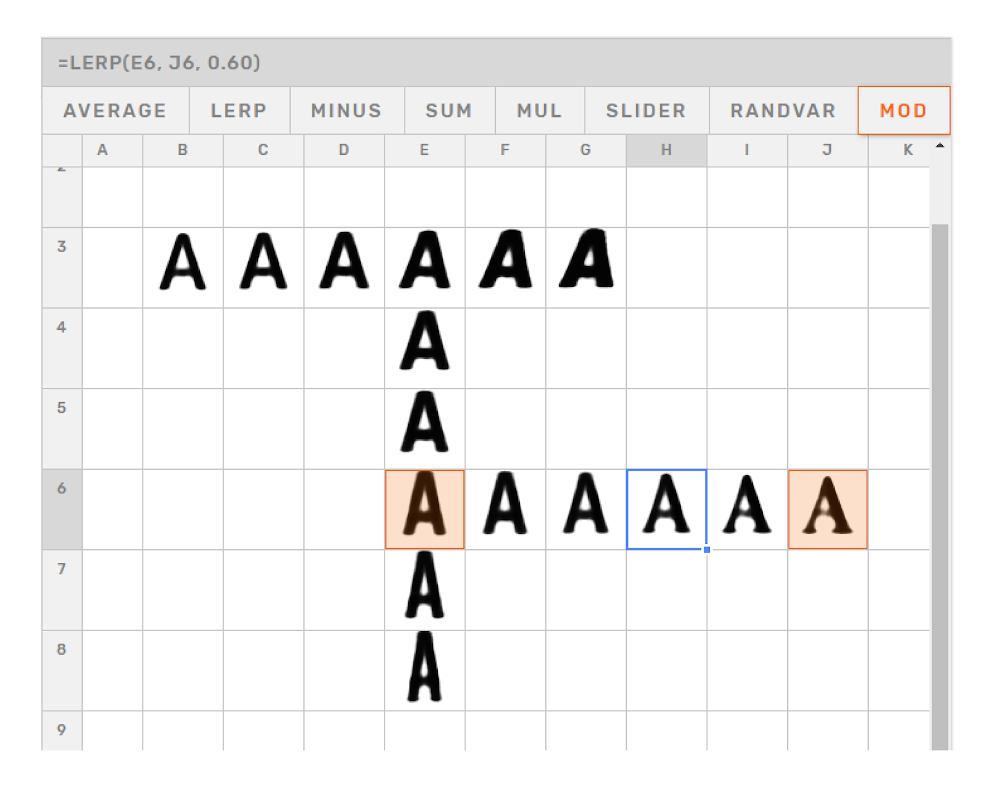
\includegraphics[width=6cm]{figs/02A-use-cases.png}
  \caption{SpaceSheet with Font Model}
\end{figure}


Initial efforts are focused on experimenting in various domains to encourage the development of a general-purpose model agnostic set of operations. A SpaceSheet to explore a generative model of fonts~\cite{bernhardsson15} has been implemented to be used as a design tool (Figure 5). User testing indicated that the tool enabled designers and non-designers alike to explore design variations easily~\cite{loh18}.

\begin{figure}[ht]
  \centering
  % \fbox{\rule[-.5cm]{0cm}{4cm} \rule[-.5cm]{4cm}{0cm}}
  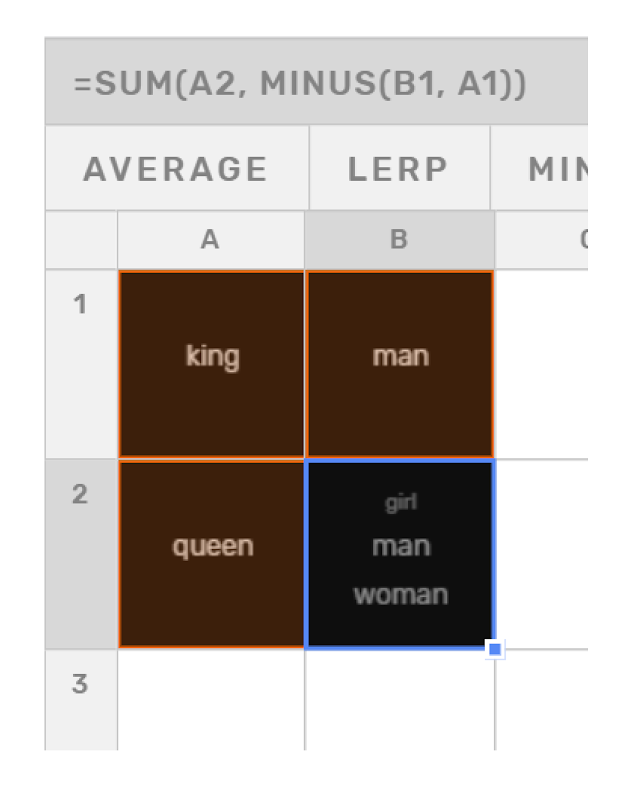
\includegraphics[width=5cm]{figs/02B-use-cases.png}
  \caption{SpaceSheet with word2vec}
\end{figure}


The concepts have also been extended to domains other than images and with models that are not generative, such as the Word2Vec model~\cite{word2vec}. This version of the SpaceSheet can be used to find word analogies and perform interpolations using nearest neighbors (Figure 6).

A SpaceSheet has been created to enable the exploration of the BigGAN model. In this implementation, the primary DataPicker for this implementation has been curated to enable users to experiment with a variety of image classes (Figure 8).

\begin{figure}[ht]
  \centering
  % \fbox{\rule[-.5cm]{0cm}{4cm} \rule[-.5cm]{4cm}{0cm}}
  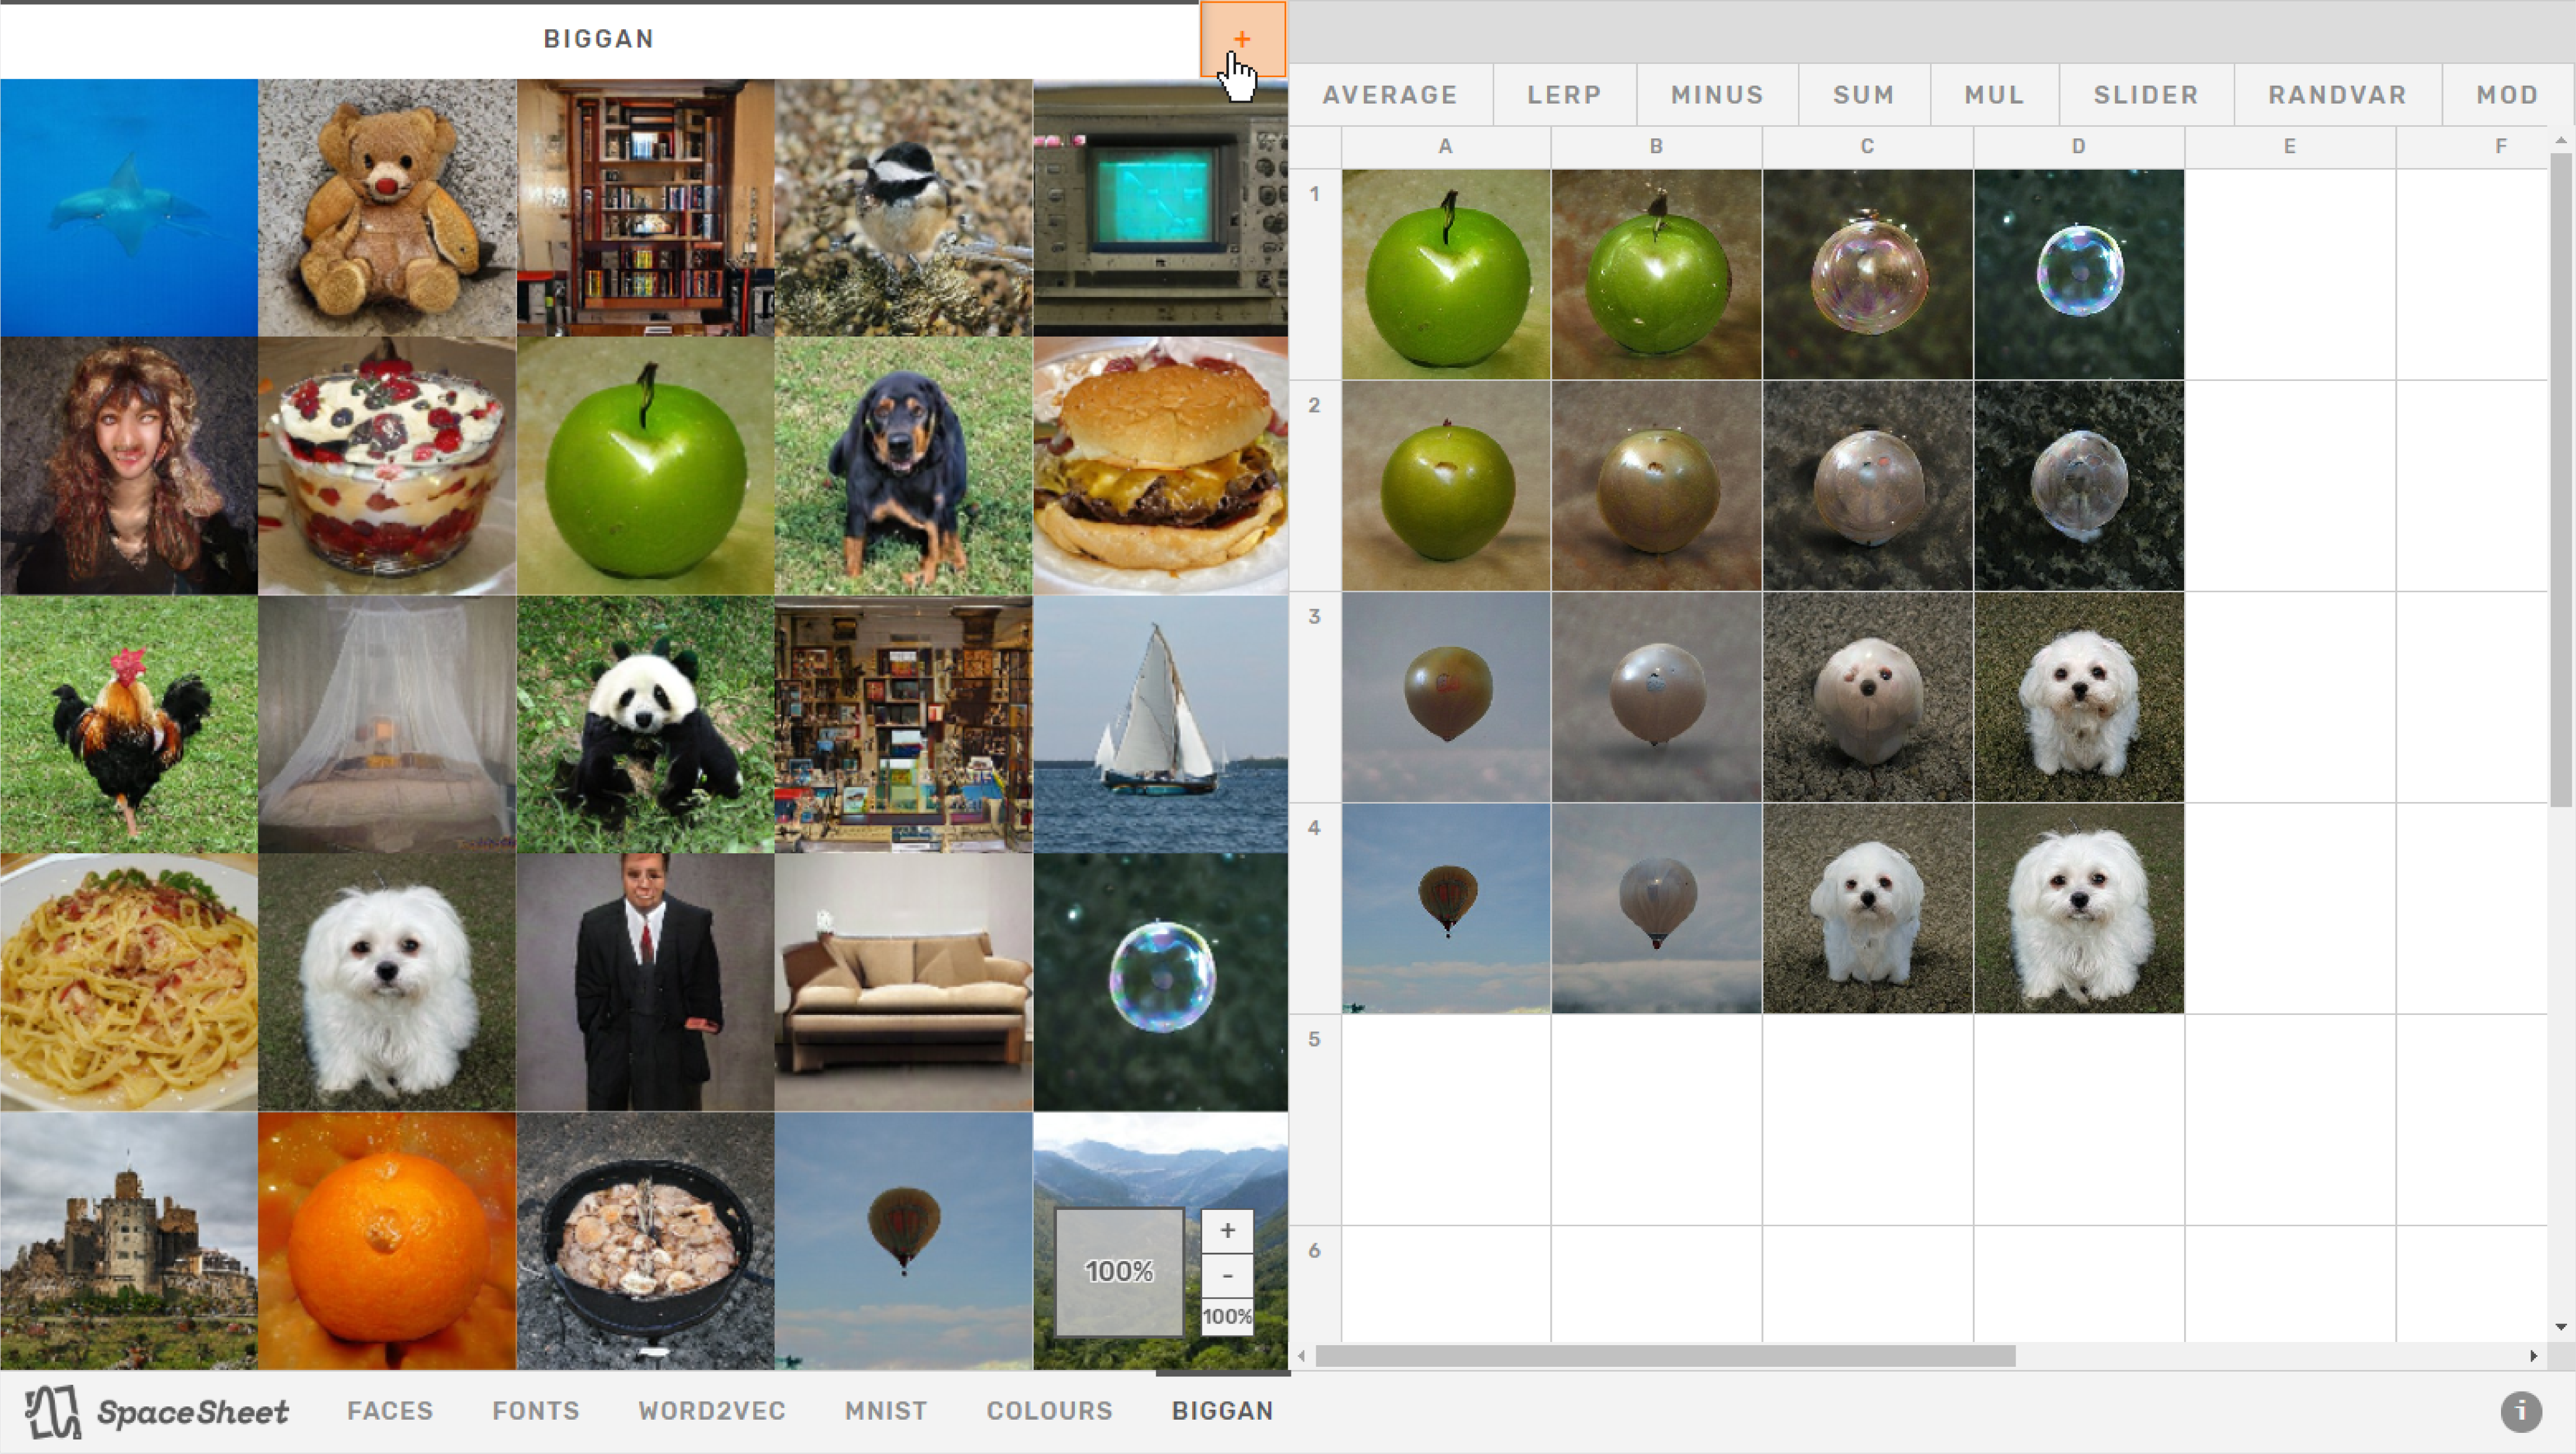
\includegraphics[width=8cm]{figs/BigGAN-01.png}
  \caption{BigGAN SpaceSheet with a generic DataPicker across all image classes}
\end{figure}

Custom DataPickers of other classes, or combinations of other classes can be created using the DataPicker creator (accessible through the highlighted button in Figure A). The DataPicker creator enables users to a) explore and select one or more classes from a searchable, hierarchically organised tree checklist, b) control the amounts of each class to composite in the resulting class, and c) preview example reconstructions of the resulting class before creating a DataPicker of the resulting class. Once created, this new custom DataPicker will be available for use in the spreadsheet (Figure 9).

\begin{figure}[ht]
  \centering
  % \fbox{\rule[-.5cm]{0cm}{4cm} \rule[-.5cm]{4cm}{0cm}}
  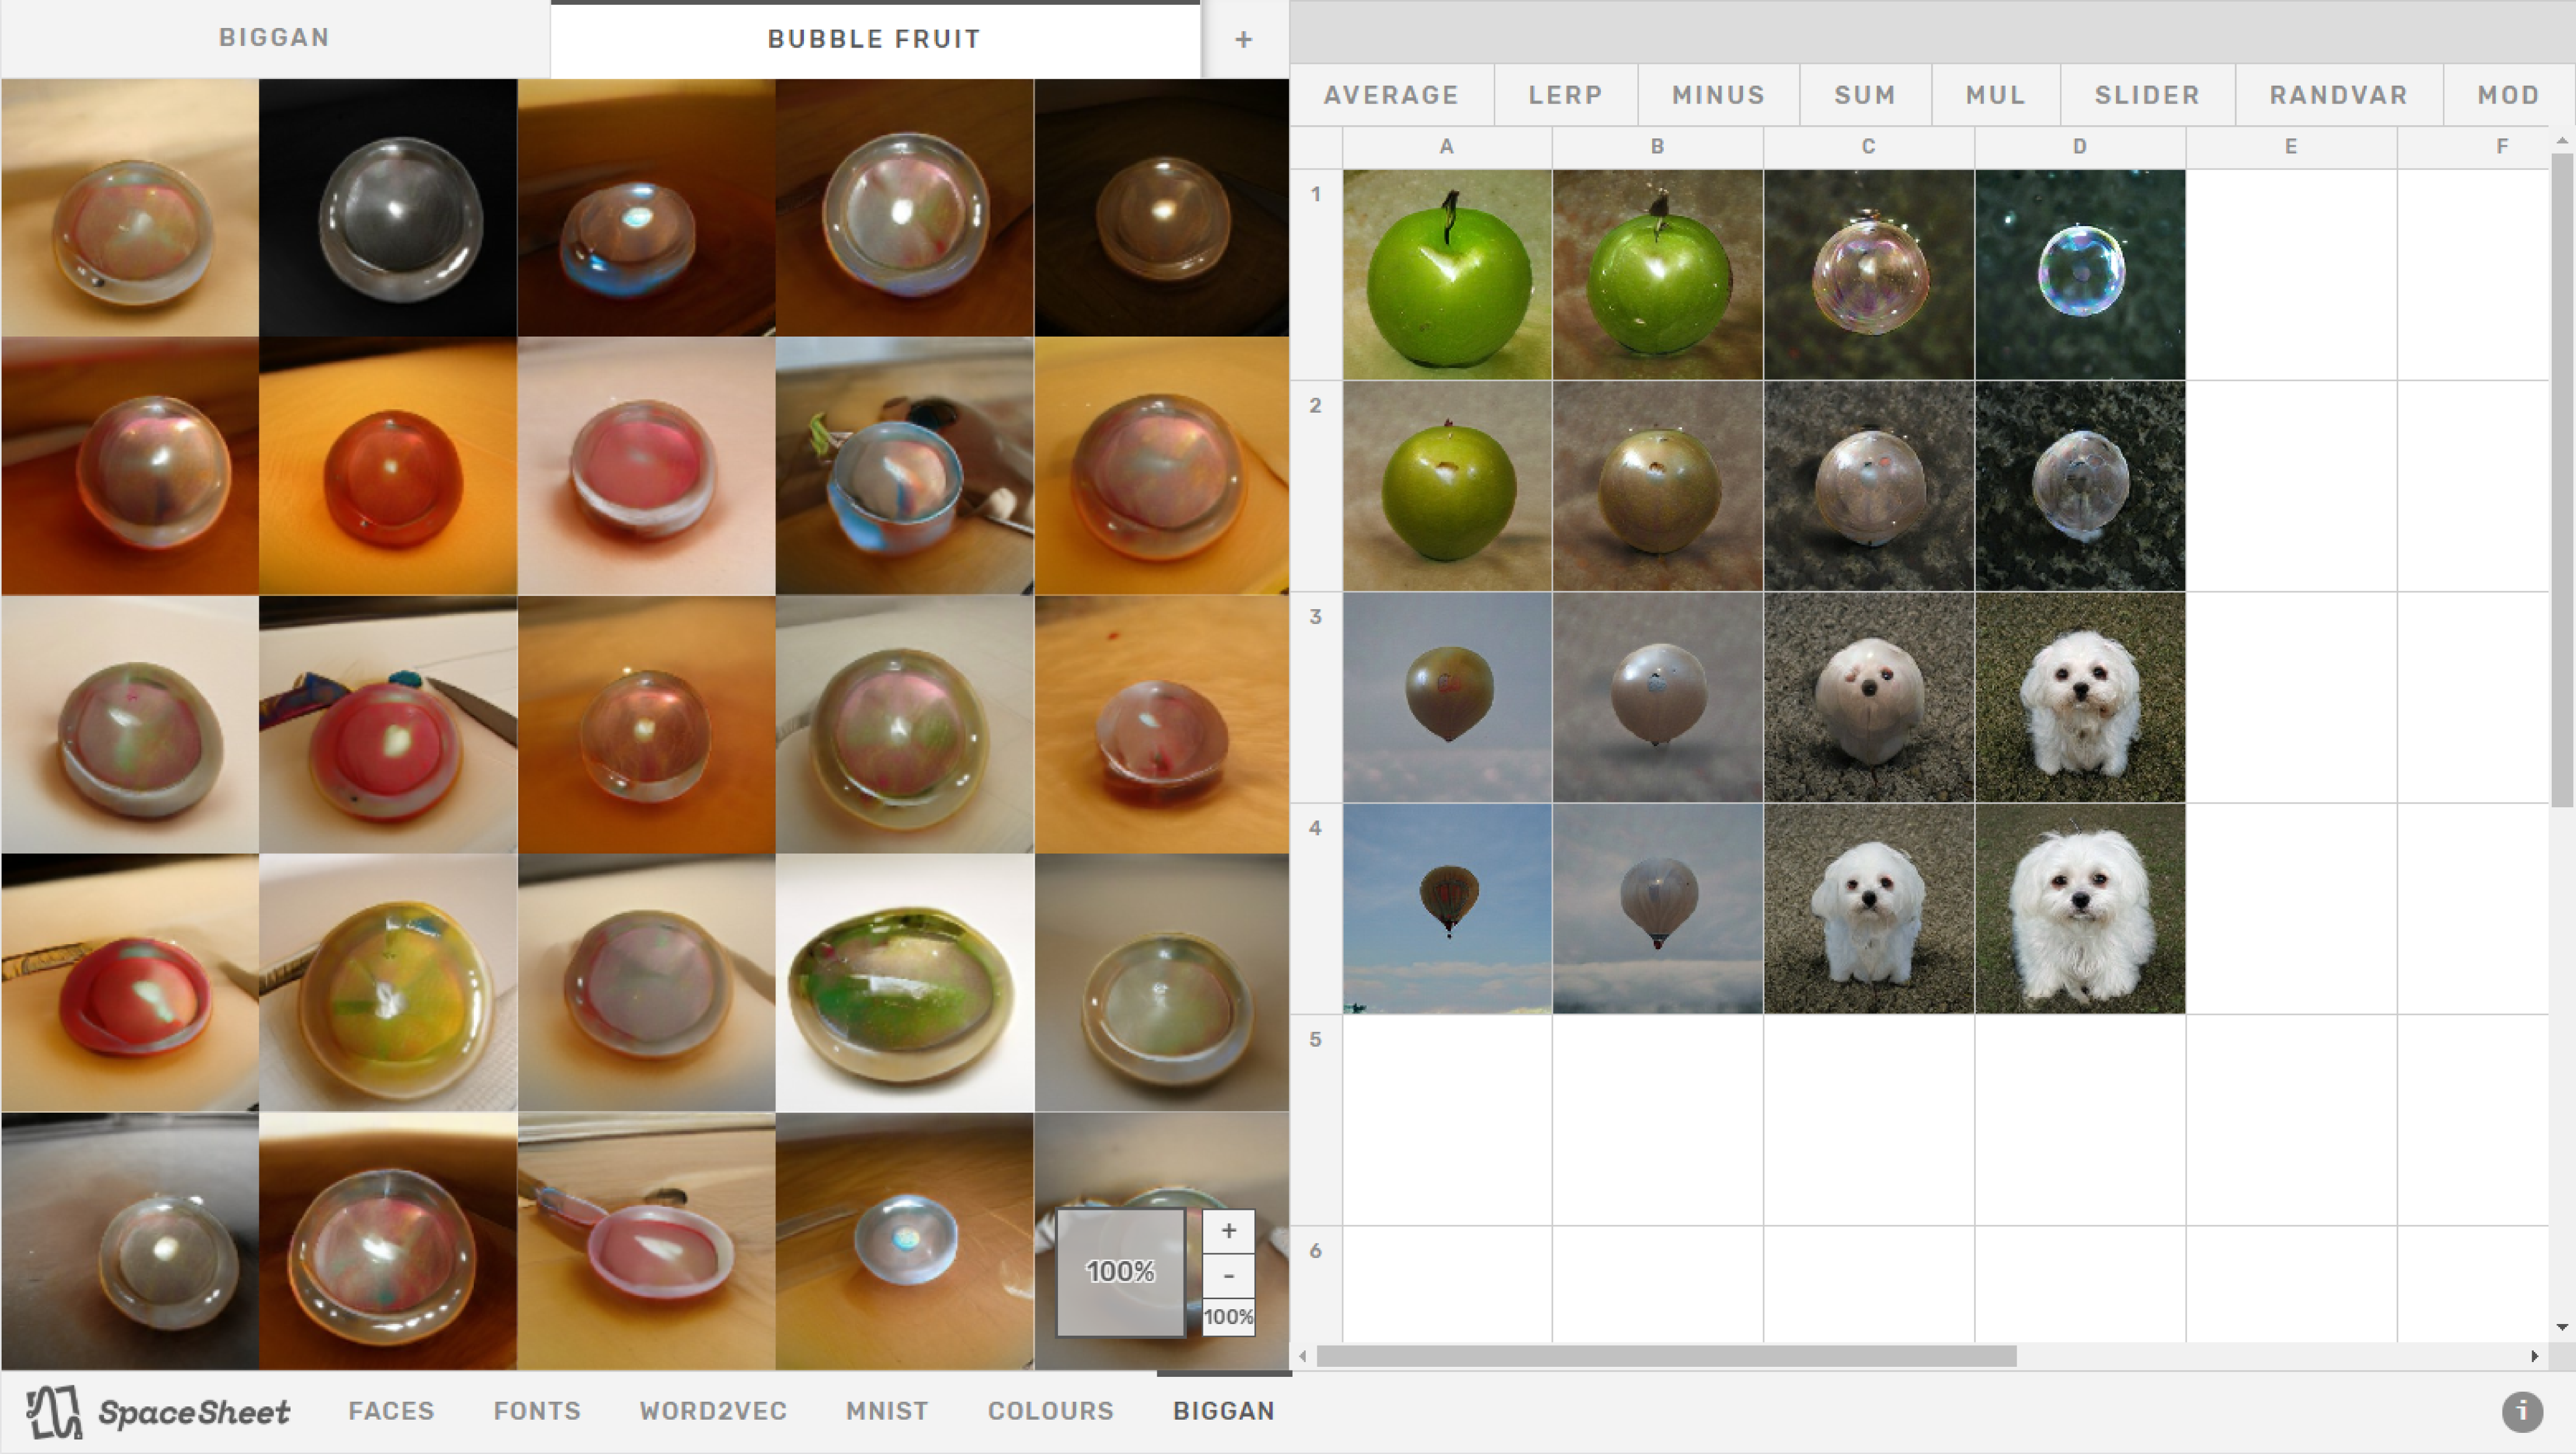
\includegraphics[width=8cm]{figs/BigGAN-03.png}
  \caption{BigGAN SpaceSheet with a custom DataPicker made from combining a user-provided ratio of the "Bubble", "Granny Smith", and "Velvet" image classes}
\end{figure}

\subsection{Evaluation}

User testing of SpaceSheets on a model of fonts~\cite{loh18} revealed that the tool enabled a novel method to experiment with designs. Users explore design possibilities from a top-down approach by deriving meaning and navigating within a preconstructed model, rather than constructing a model from the bottom-up.

This method of working was reported to be more supportive of design exploration, more efficient, and capable of enabling non-designers to explore design possibilities. Unsurprisingly, it required new skills and intuition to be used to its full effect. A lack of knowledge in deriving and applying attribute vectors from latent space limited users’ expressivity and control over their experiments. Due to this, interpolation was found to be the most intuitive and common method to arrive at search targets.

Expressing low-level transformations such as positioning and scale through SpaceSheet often resulted in distorted reconstructions which did not match the expectations of the user. This is attributed to a mismatch in the high-level probabilism of sampling latent spaces is an ill-fit to express concrete design intent. However, this uncertainty has been reported to be serendipitous when distortions in the reconstruction added to the aesthetics of the design.

\subsection{Discussion}

SpaceSheets explores the potential of latent spaces to be used as a tool for design experimentation. The research finds it to enable a novel method to work with designs which supports more efficient, high-level design experimentation to designers and non-designers alike. 

User intuition and skill in deriving meaning from latent spaces is fundamental to conduct design experiments with a fine level of control. This intuition can be considered a skill which can be developed through continued experience with the flexible, low-level interface provided by the SpaceSheet. Although latent spaces enable designers to express more meaningful design operations computationally, it provides redundant uncertainty for low-level design operations. It is with this understanding that latent spaces are best considered as a complementary new primitive to build smarter design tools.

\bibliographystyle{iccc}
\bibliography{iccc,spacesheet}

\onecolumn

\pagebreak

\normalsize

% \vspace*{0.15\textheight}

\section*{Appendix: Implementation Details}

\section*{Supported Operations}

\renewcommand{\arraystretch}{1.5}

\begin{center}
    \begin{tabular}{ | l | p{6cm} | p{5.6cm} |}
    \hline \textbf{Operation} & \textbf{Description} & \textbf{Formula} \\ \hline
    Sum & Adds a list of numbers / variables  & \texttt{SUM(val1, val2, val3, ...)} \\ \hline
    Minus & Subtracts two numbers / variables in sequence  & \texttt{MINUS(val1, val2)} \\ \hline
    Multiply & Multiplies a list of numbers / variables  & \texttt{MUL(val1, val2, val3, ...)} \\ \hline
    Linear Interpolation & Calculates the value in between two numbers / vectors at a specified amount  & \texttt{LERP(from, to, amount)} \\ \hline
    Average & Calculates the average of a list of numbers / vectors  & \texttt{AVERAGE(val1, val2, val3, ...)} \\ \hline
    Distance & Calculates the euclidean distance between two numbers / vectors  & \texttt{DIST(val1, val2)} \\ \hline
    Modulate & Creates a scrubbing interface which can modulate a cell  & \texttt{MOD(cell, degree, radius)} \\ \hline
    Random Variable & Creates a random latent variable  & \texttt{RANDVAR(seed)} \\ \hline
    Slider & Creates a number which is controlled by a slider element  & \texttt{SLIDER(min, max[, step])} \\ \hline
    \end{tabular}
\end{center}


\section*{Interactive Cell Types}

\begin{figure}[ht!]
  \centering
  % \fbox{\rule[-.5cm]{0cm}{4cm} \rule[-.5cm]{4cm}{0cm}}
  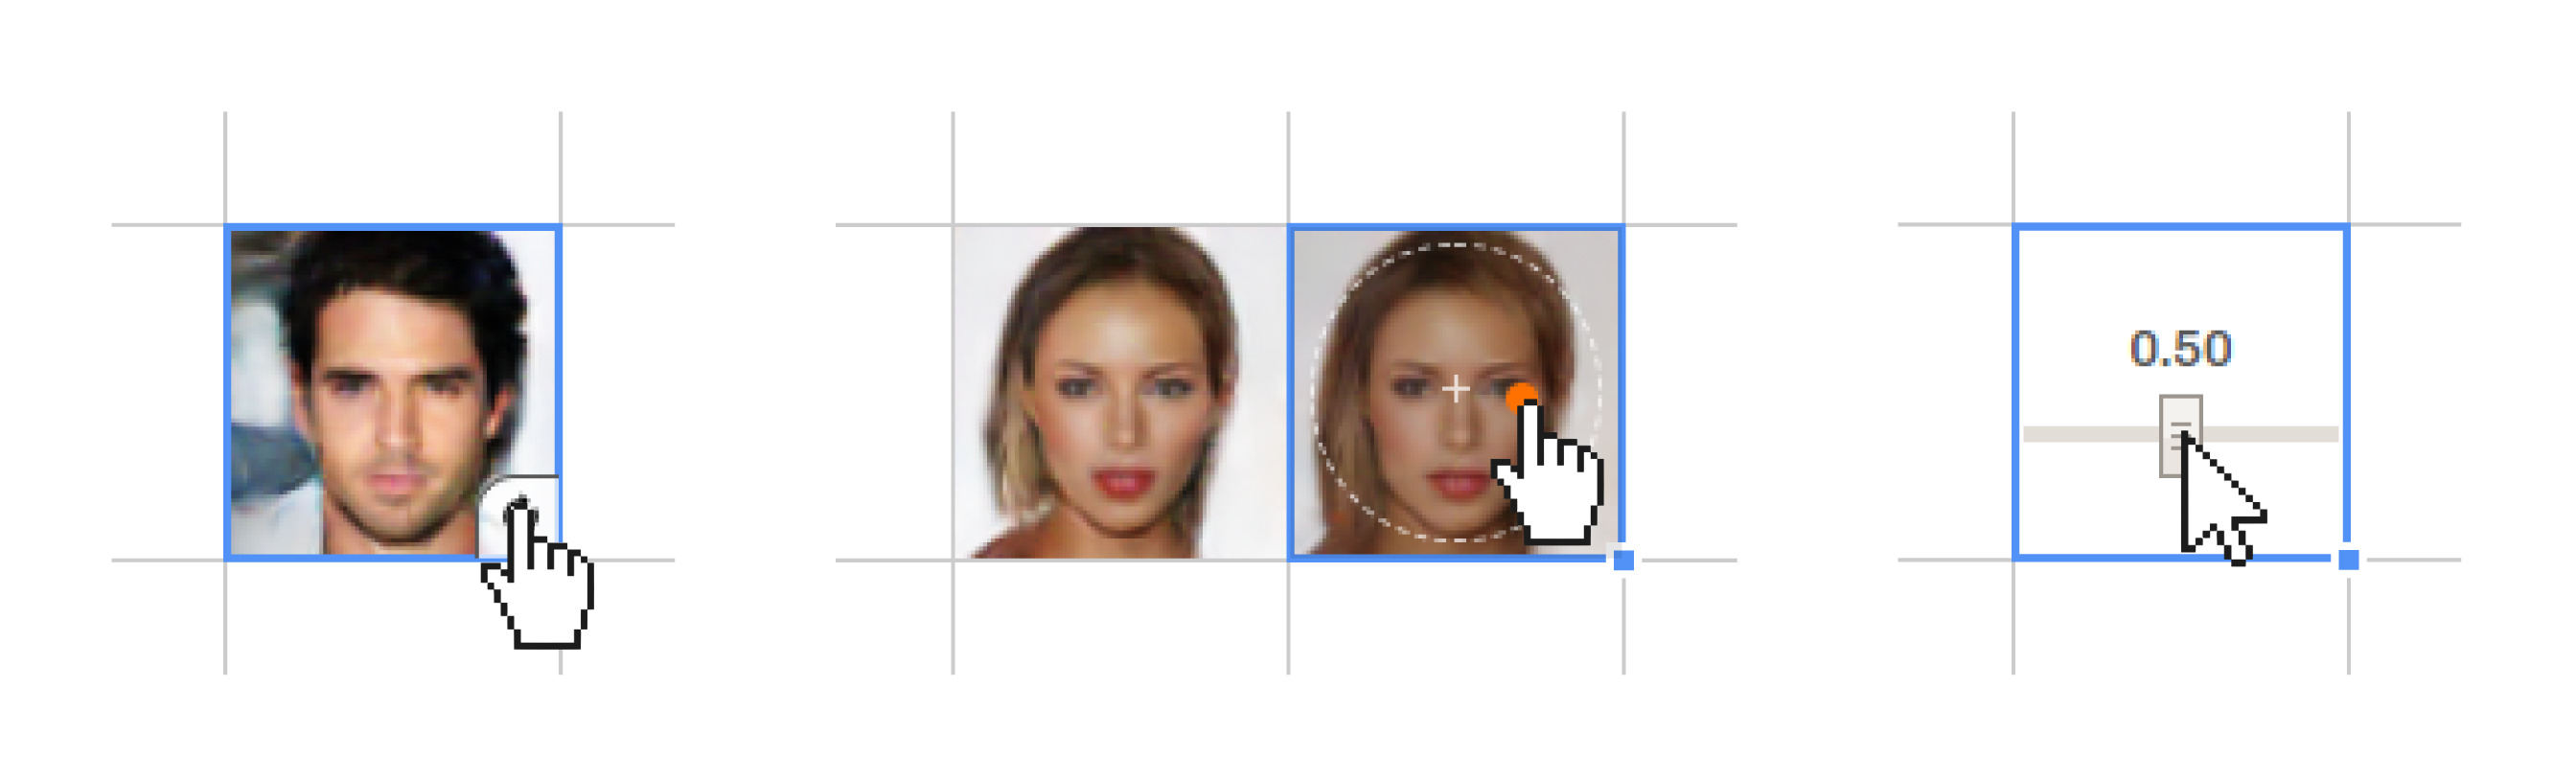
\includegraphics[width=12cm]{figs/03-cell-types.jpg}
  \caption{RANDVAR, MOD and SLIDER cells.}
\end{figure}

Several alternative cell types have been implemented to create interface elements which support more effective search and exploration. These are instantiated by the operations:

\begin{verbatim}
RANDVAR(seed)
\end{verbatim}
The RANDVAR (random variable) cell instantiates a latent variable from a random seed. This enables users to operate using latent variables beyond the limited set afforded by the Data Picker. A button displays when the cell is hovered over which enables users to randomise the cell directly.

\begin{verbatim}
MOD(base, degree, distance)
\end{verbatim}
The MOD (modulate) cell exposes a joystick interface which enables users to scrub locally around a given latent variable to arrive at similar latent variables. The degree of difference can be controlled by the joystick’s distance from the center of the cell.

\begin{verbatim}
SLIDER(min, max [,step])
\end{verbatim}
The slider cell enables users to create a number controlled by a slider element.

\newpage 
\section*{Example Workflows}

% turn off subsection numbering
\setcounter{secnumdepth}{0}

\subsection{Interpolation}
\begin{figure}[ht!]
  \centering
  % \fbox{\rule[-.5cm]{0cm}{4cm} \rule[-.5cm]{4cm}{0cm}}
  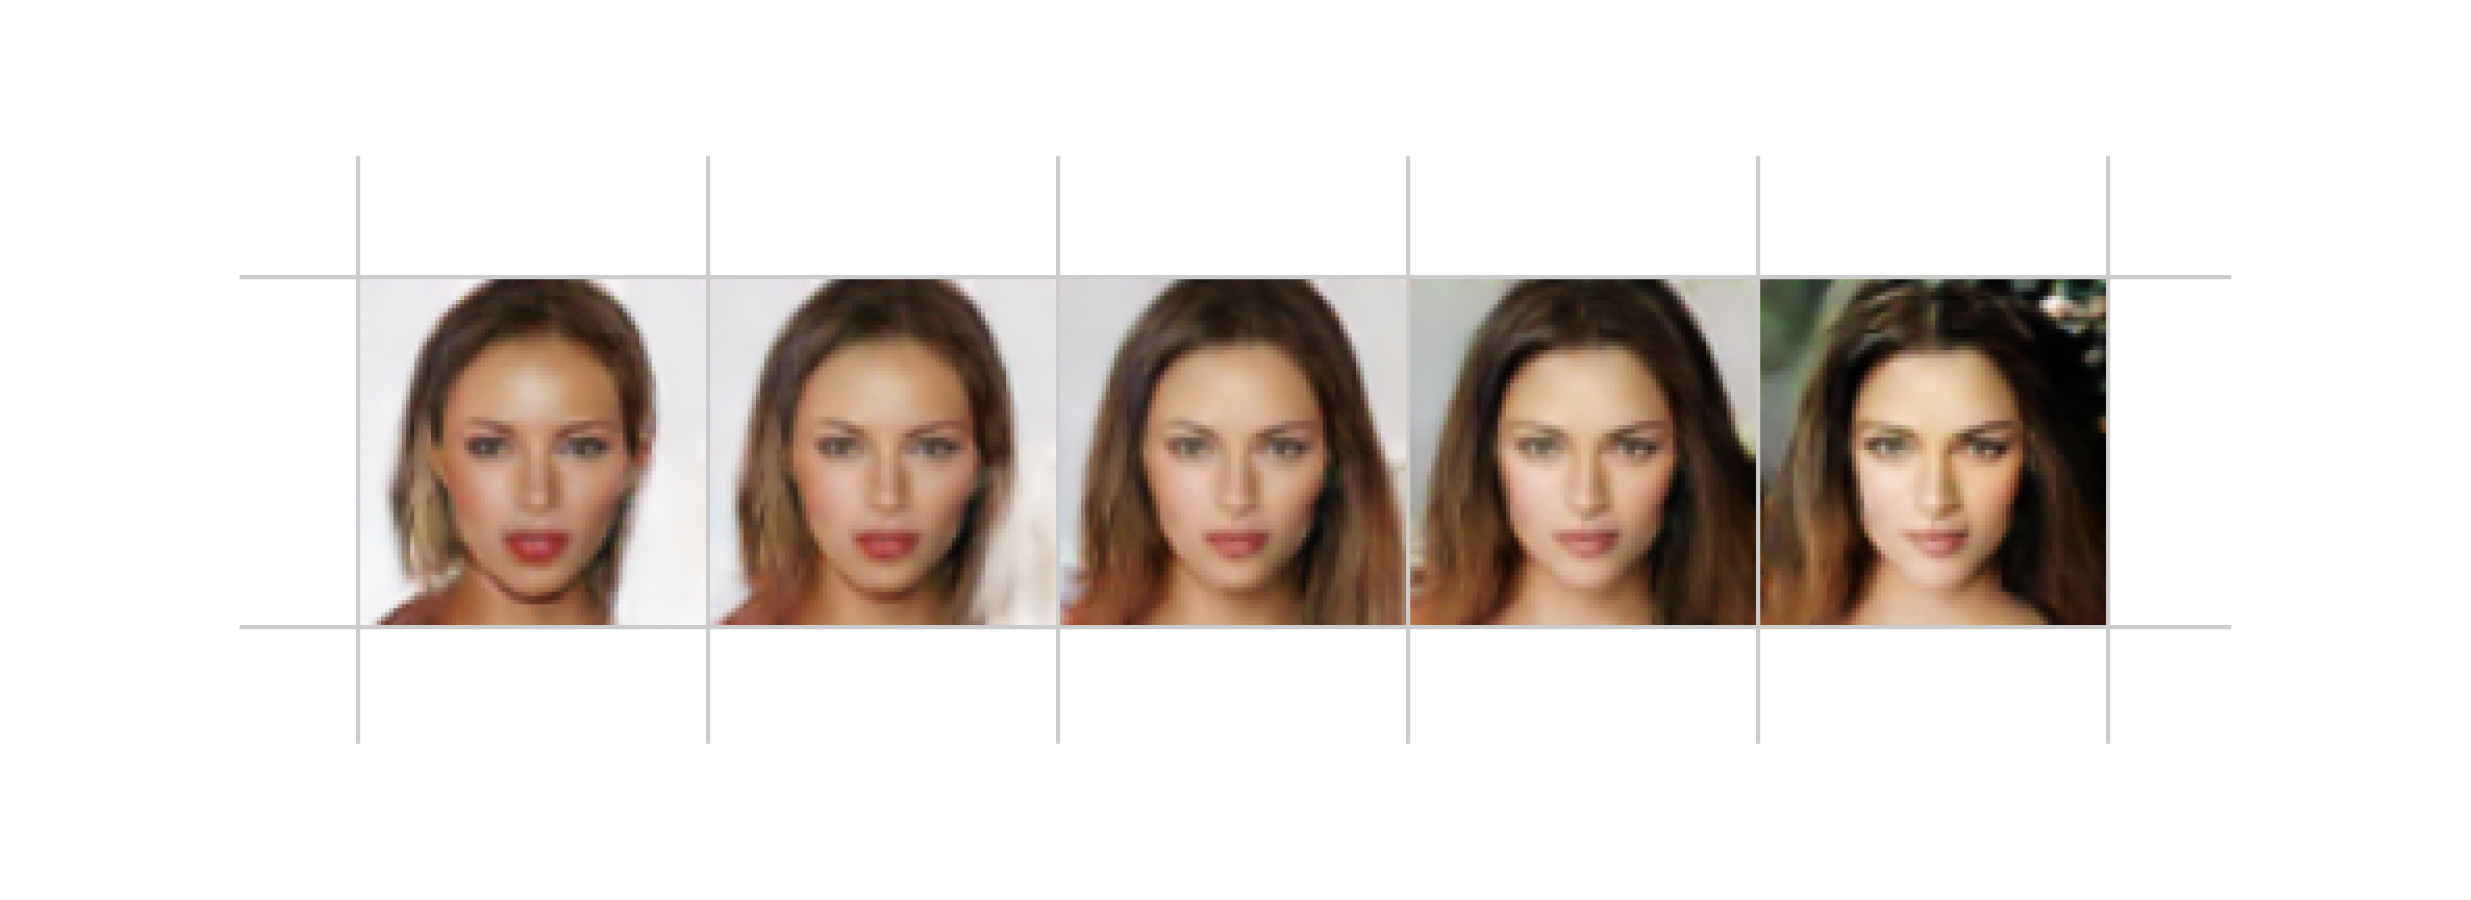
\includegraphics[width=7.5cm]{figs/04-interpolation-strip.jpg}
  \caption{An interpolation between two latent variables}
\end{figure}

\subsection{Interpolation Strip - Slider Control}
\begin{figure}[ht!]
  \centering
  % \fbox{\rule[-.5cm]{0cm}{4cm} \rule[-.5cm]{4cm}{0cm}}
  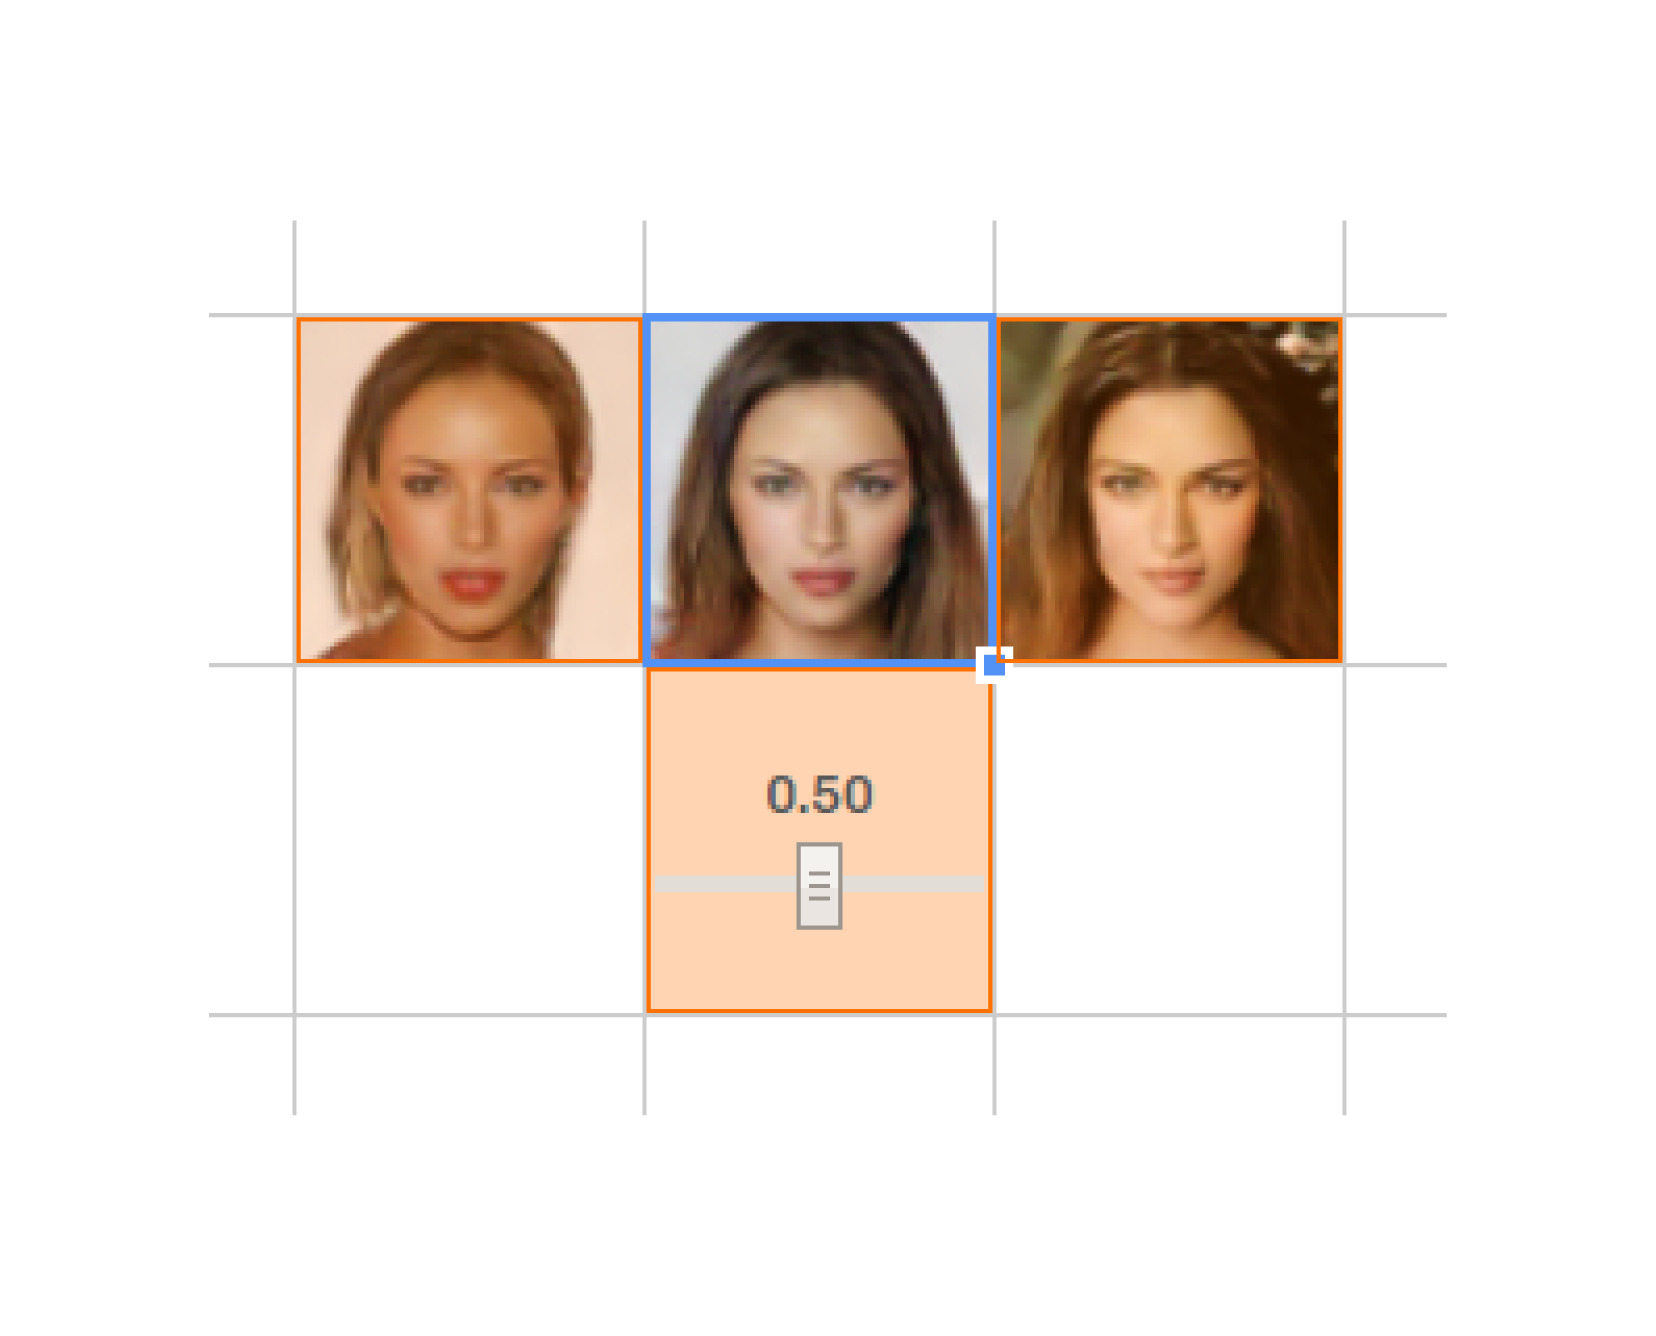
\includegraphics[width=6cm]{figs/05-interpolation-by-slider.jpg}
  \caption{An interpolation between two latent variables controlled using a slider cell}
\end{figure}

\subsection{Interpolation Grid - Four Corners}
\begin{figure}[ht!]
  \centering
  % \fbox{\rule[-.5cm]{0cm}{4cm} \rule[-.5cm]{4cm}{0cm}}
  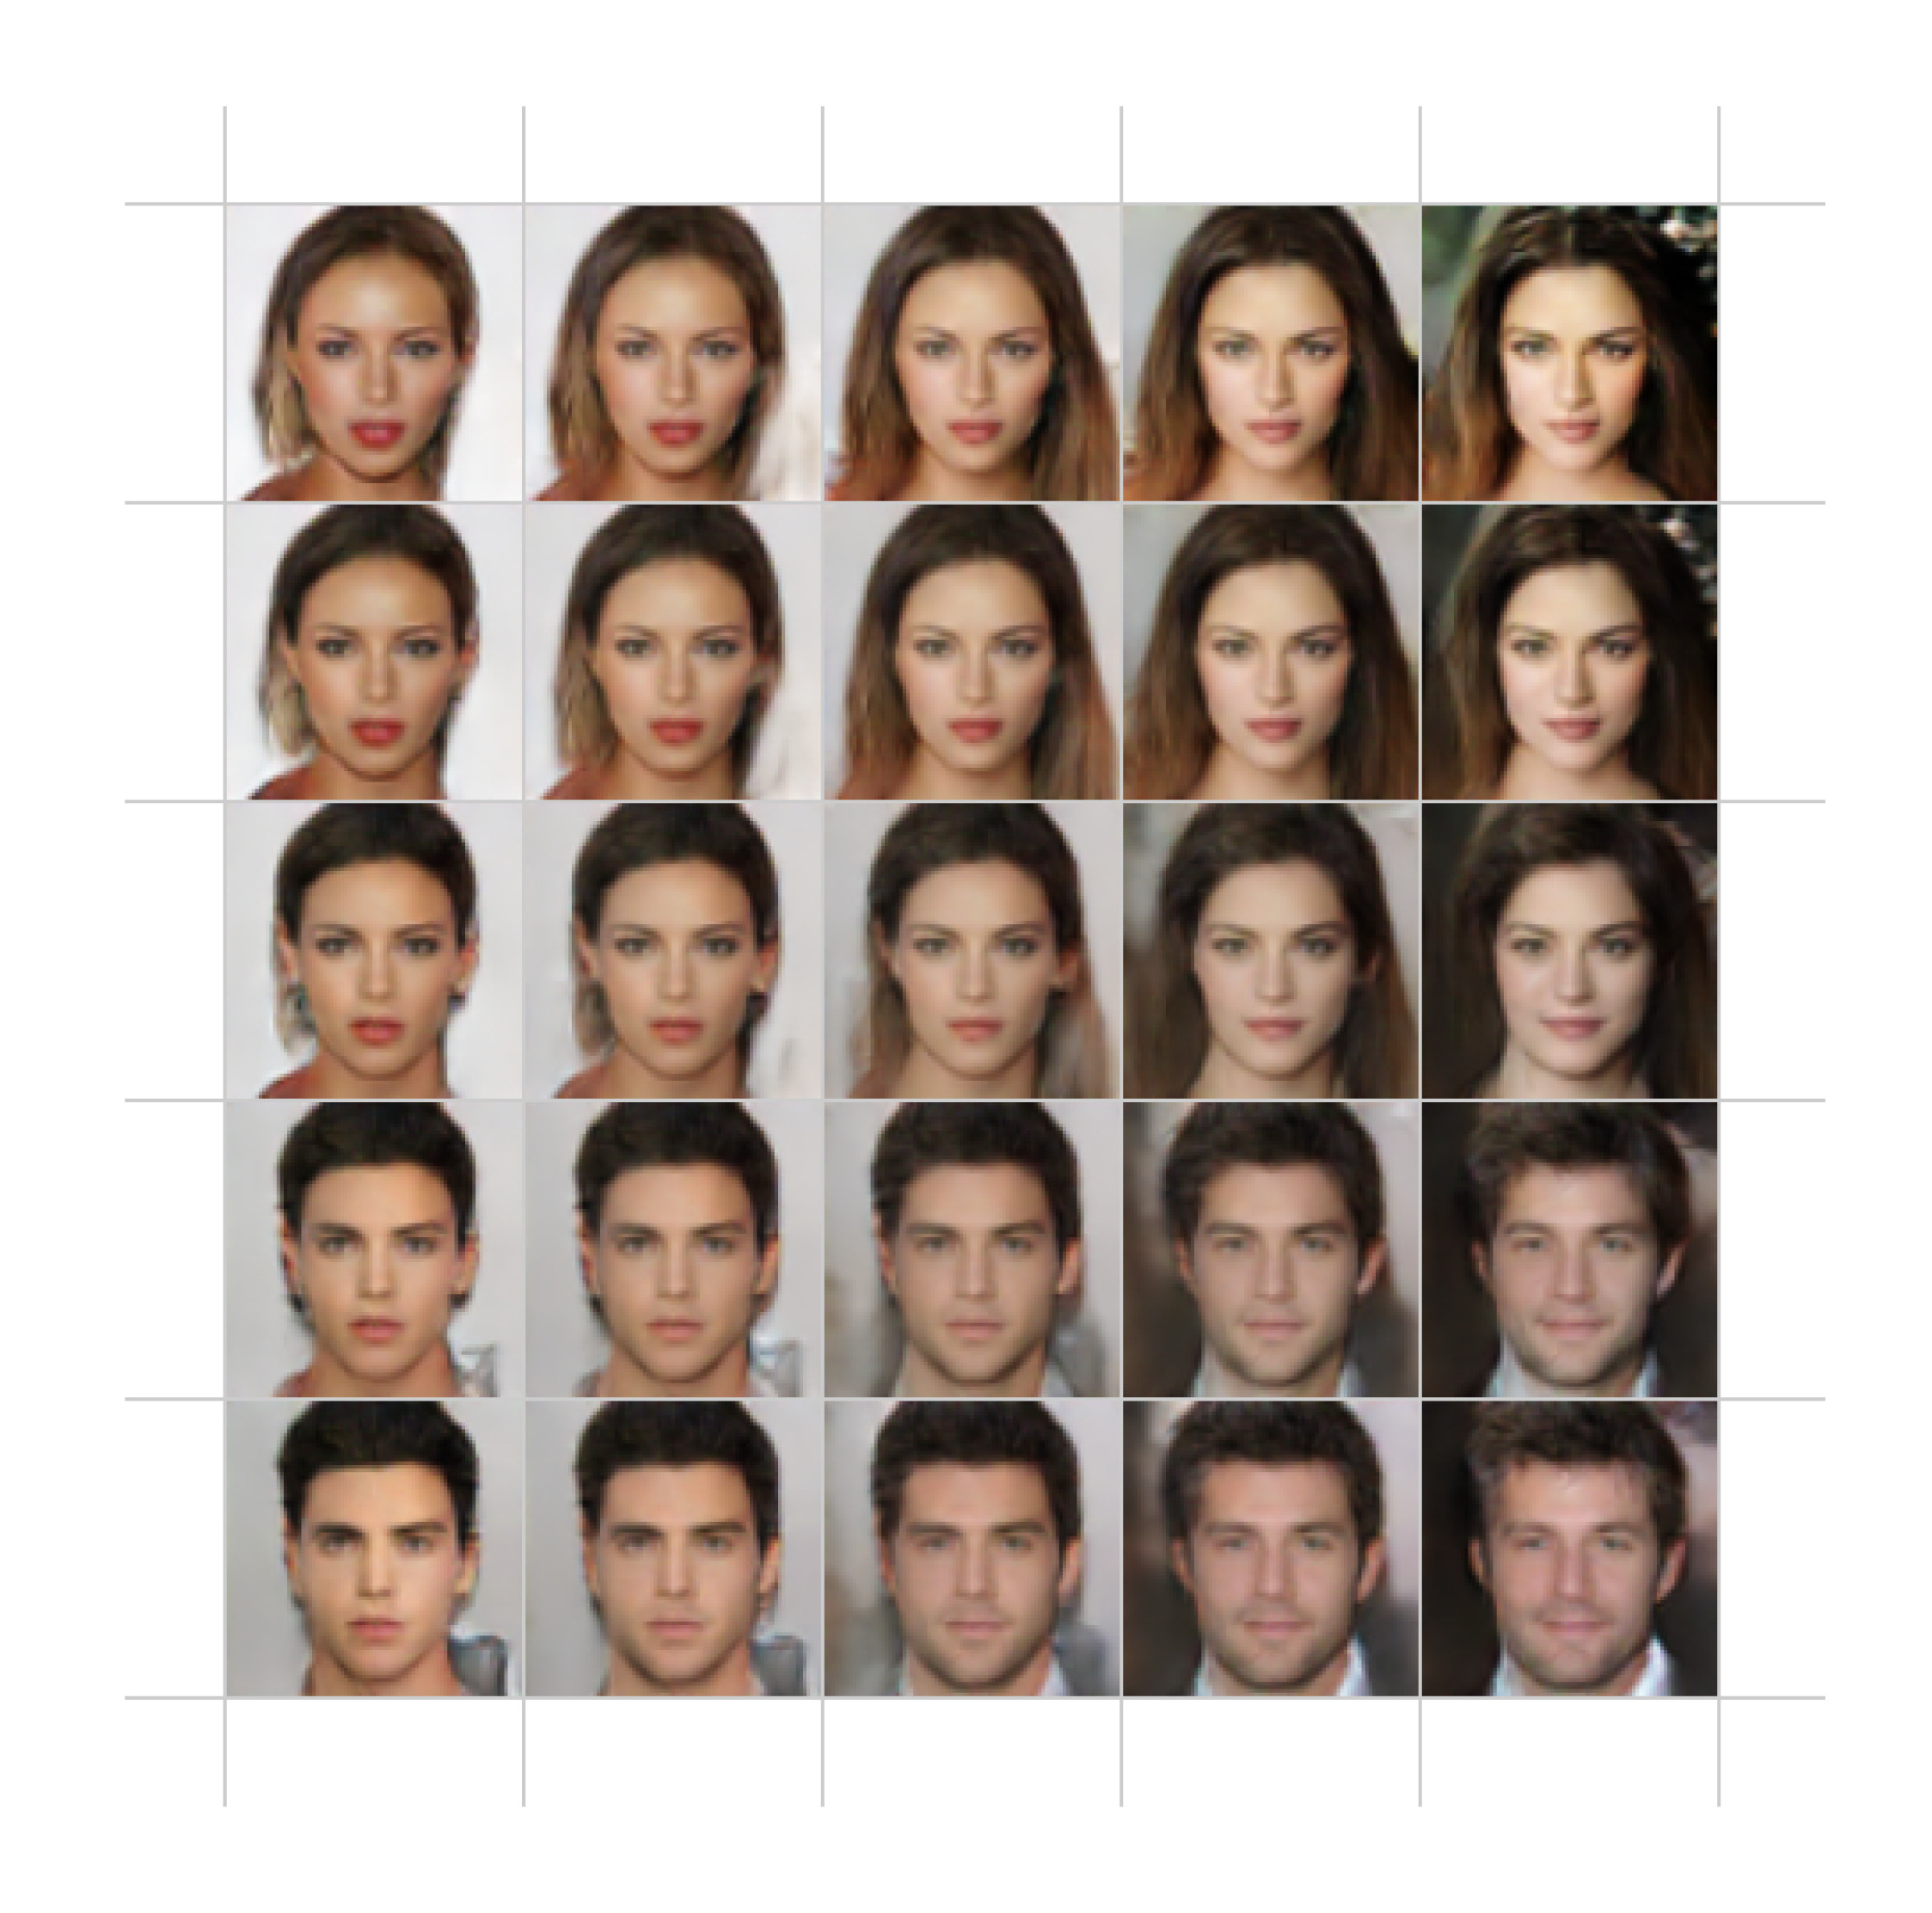
\includegraphics[width=7.5cm]{figs/06-interpolation-grid.jpg}
  \caption{An interpolation between four latent variables}
\end{figure}

\newpage 
\subsection{Analogy}
\begin{figure}[ht!]
  \centering
  % \fbox{\rule[-.5cm]{0cm}{4cm} \rule[-.5cm]{4cm}{0cm}}
  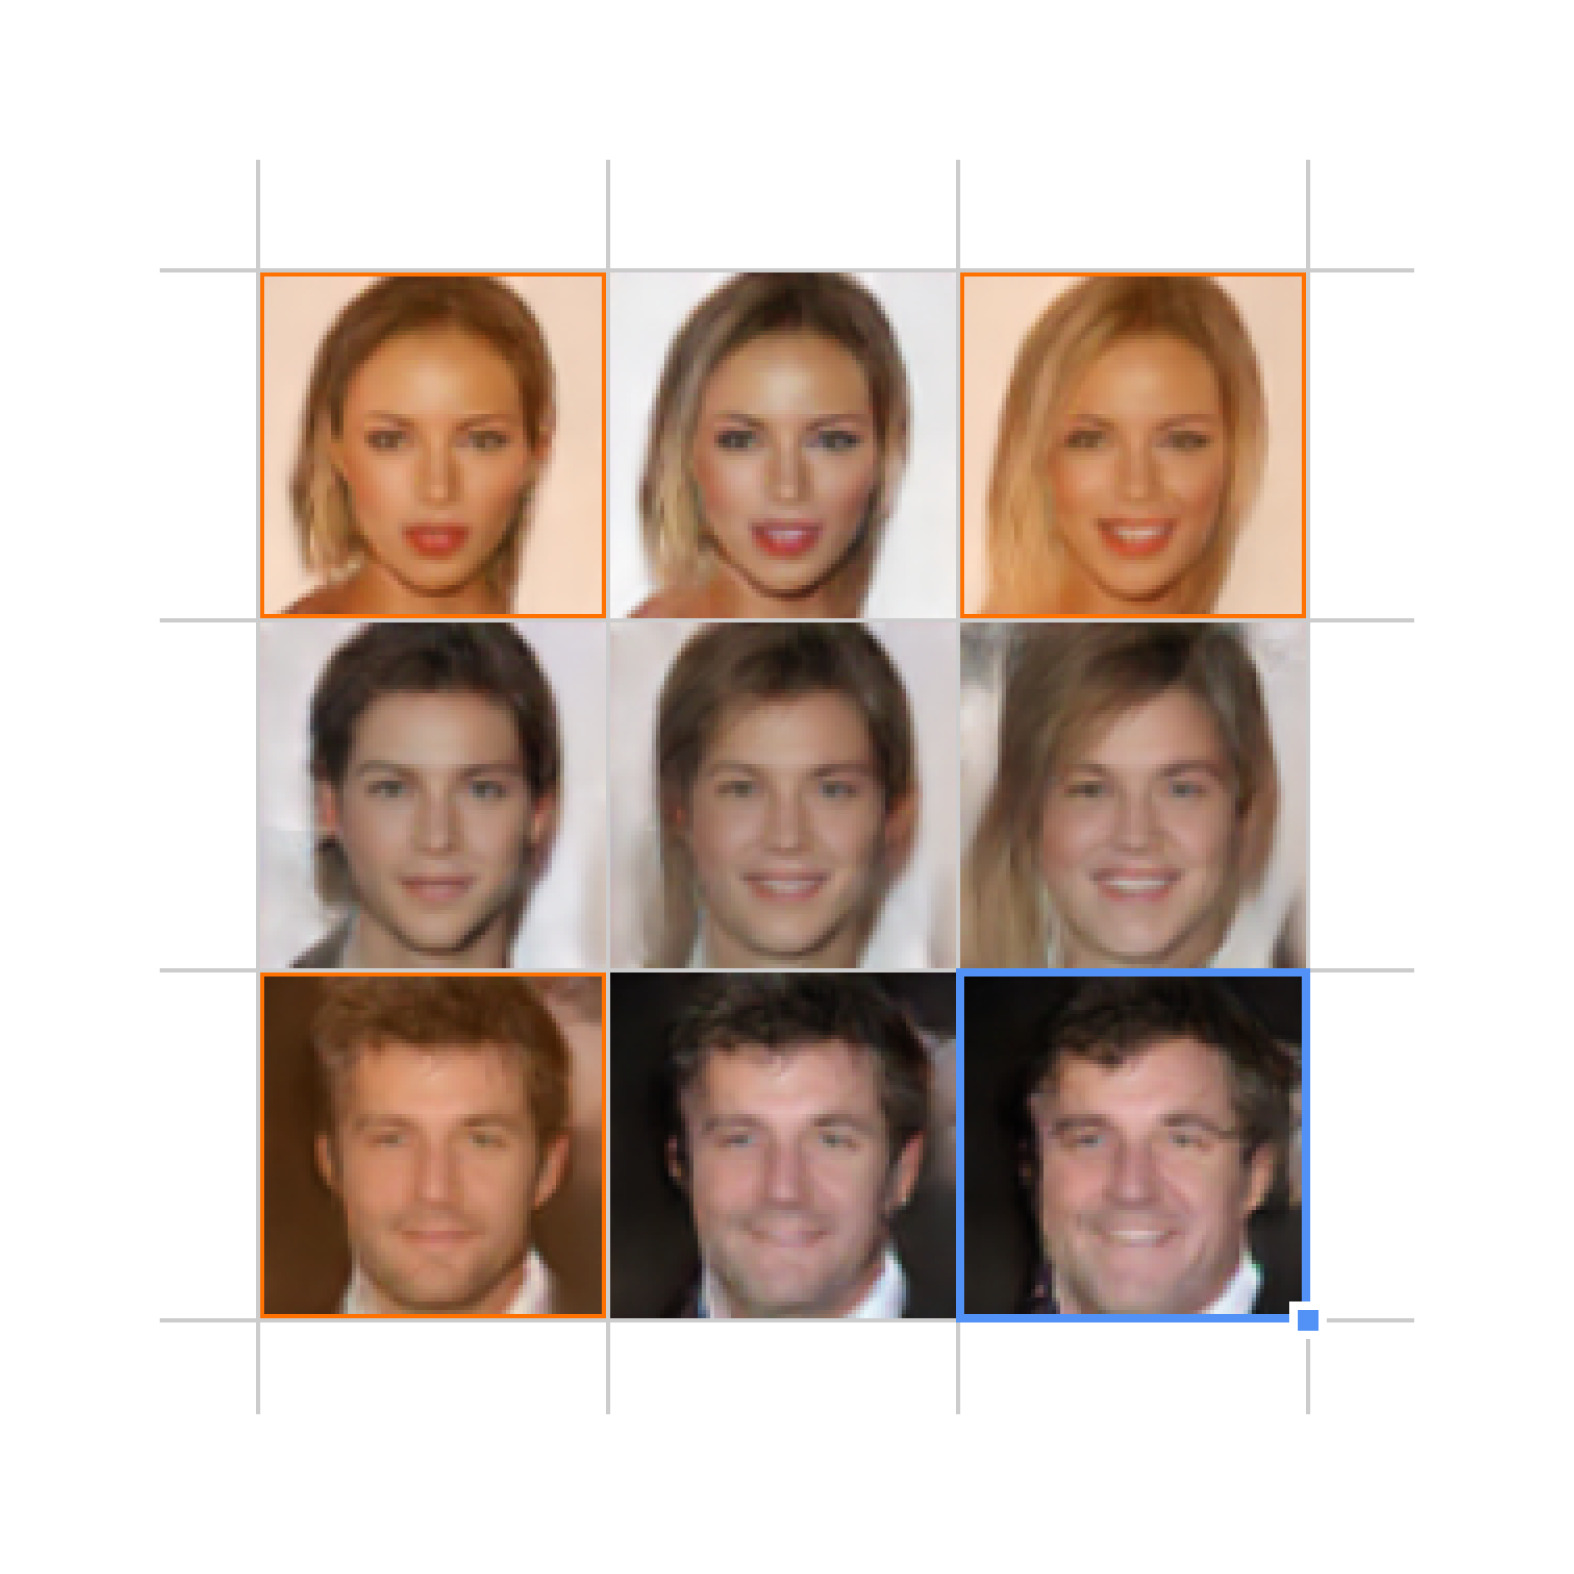
\includegraphics[width=5.5cm]{figs/07-analogy.jpg}
  \caption{An analogical construction. The bottom right cell applies the difference between the top cells to the cell on the bottom-left}
\end{figure}

Given three reconstructions (top-left, top-right, bottom-left), the SpaceSheet calculates the bottom-right corner by analogy. This is achieved by applying the difference between the top variables to the bottom-left variable. In this example, a toothy grin has been applied to the man.

\subsection{Extrapolation}
\begin{figure}[ht!]
  \centering
  % \fbox{\rule[-.5cm]{0cm}{4cm} \rule[-.5cm]{4cm}{0cm}}
  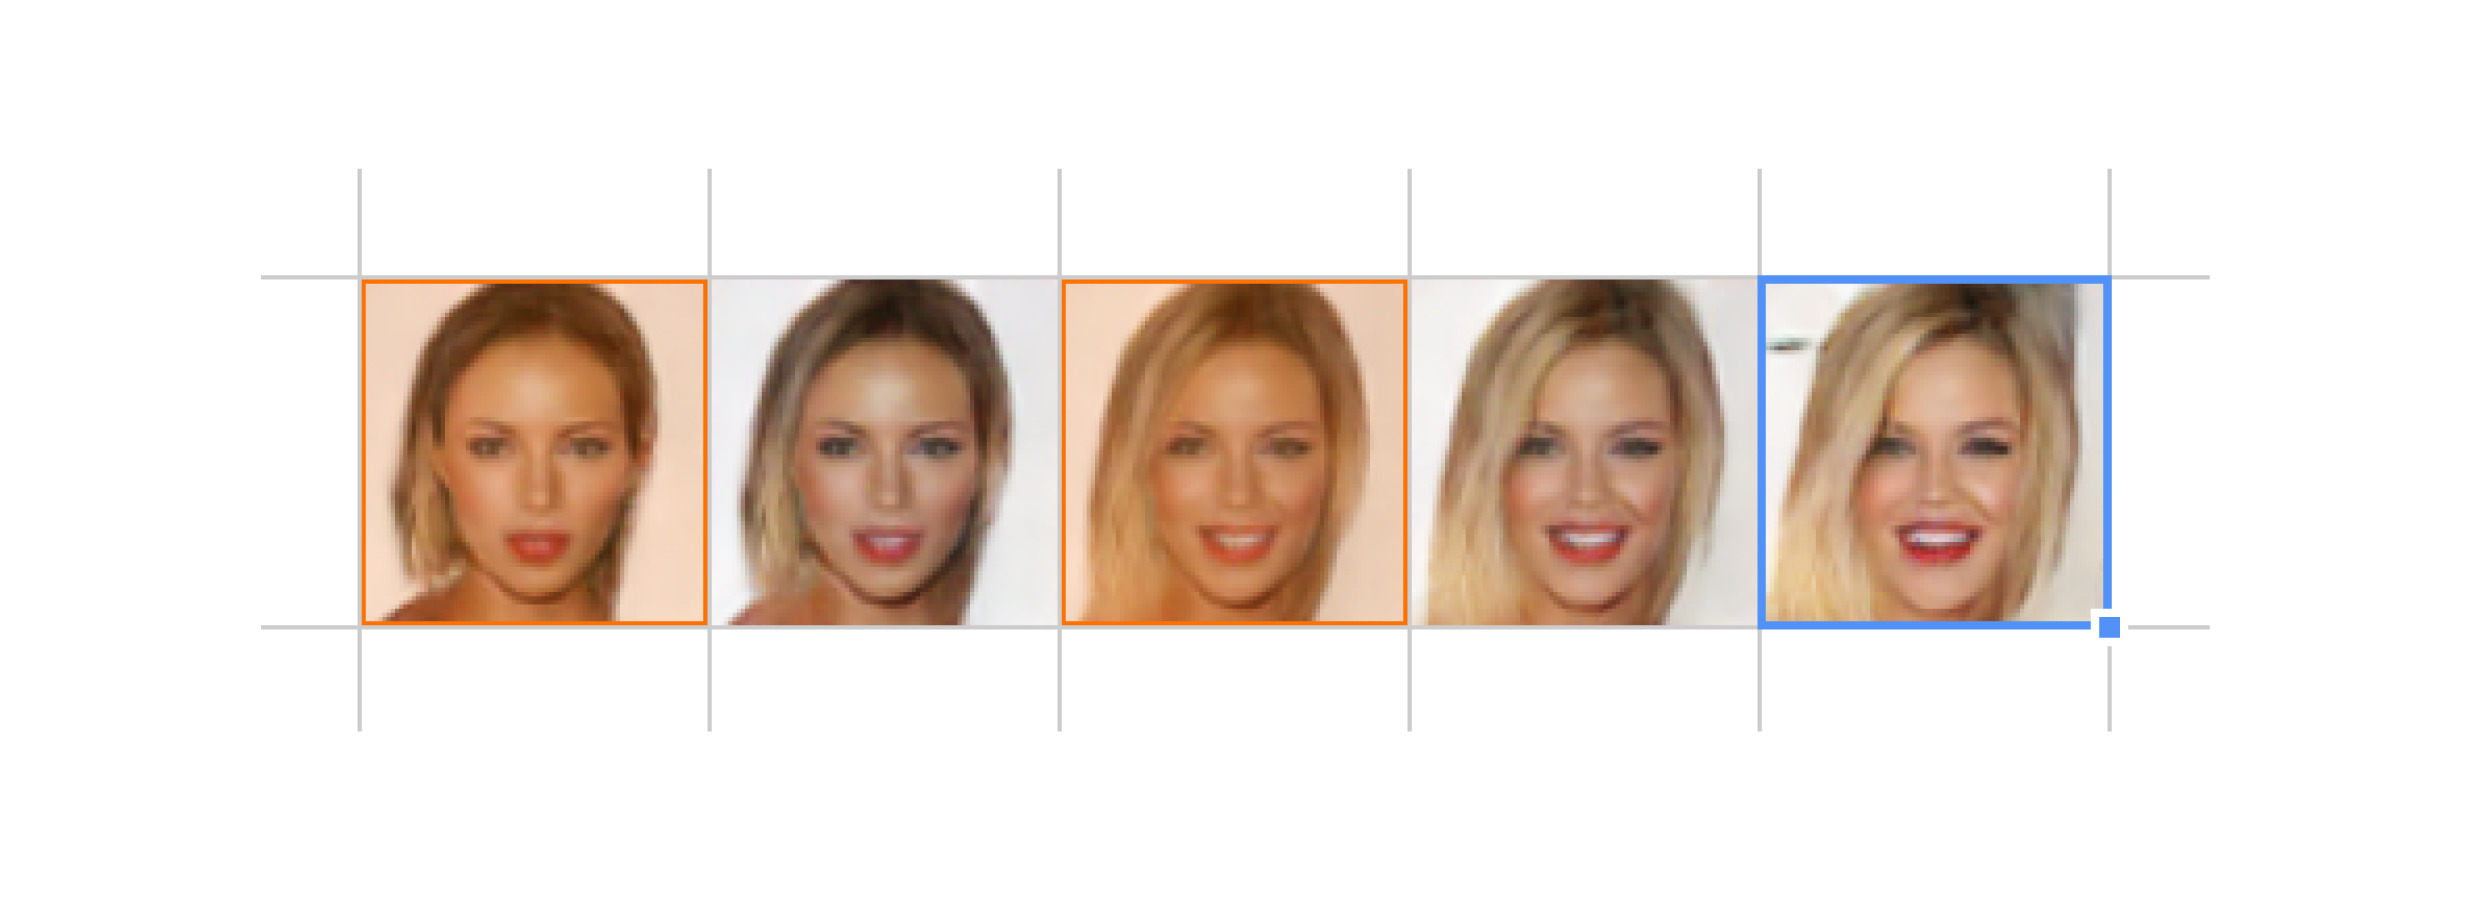
\includegraphics[width=8cm]{figs/08-extrapolation.jpg}
  \caption{Extrapolating from two points.}
\end{figure}

Extrapolating from latent variables can be used to emphasise attributes which vary between its anchors. In this example, the difference between the highlighted anchors - blond hair, large smile, etc.  - have been emphasised by extrapolating beyond the end anchor.

\subsection{Averaging}
\begin{figure}[ht!]
  \centering
  % \fbox{\rule[-.5cm]{0cm}{4cm} \rule[-.5cm]{4cm}{0cm}}
  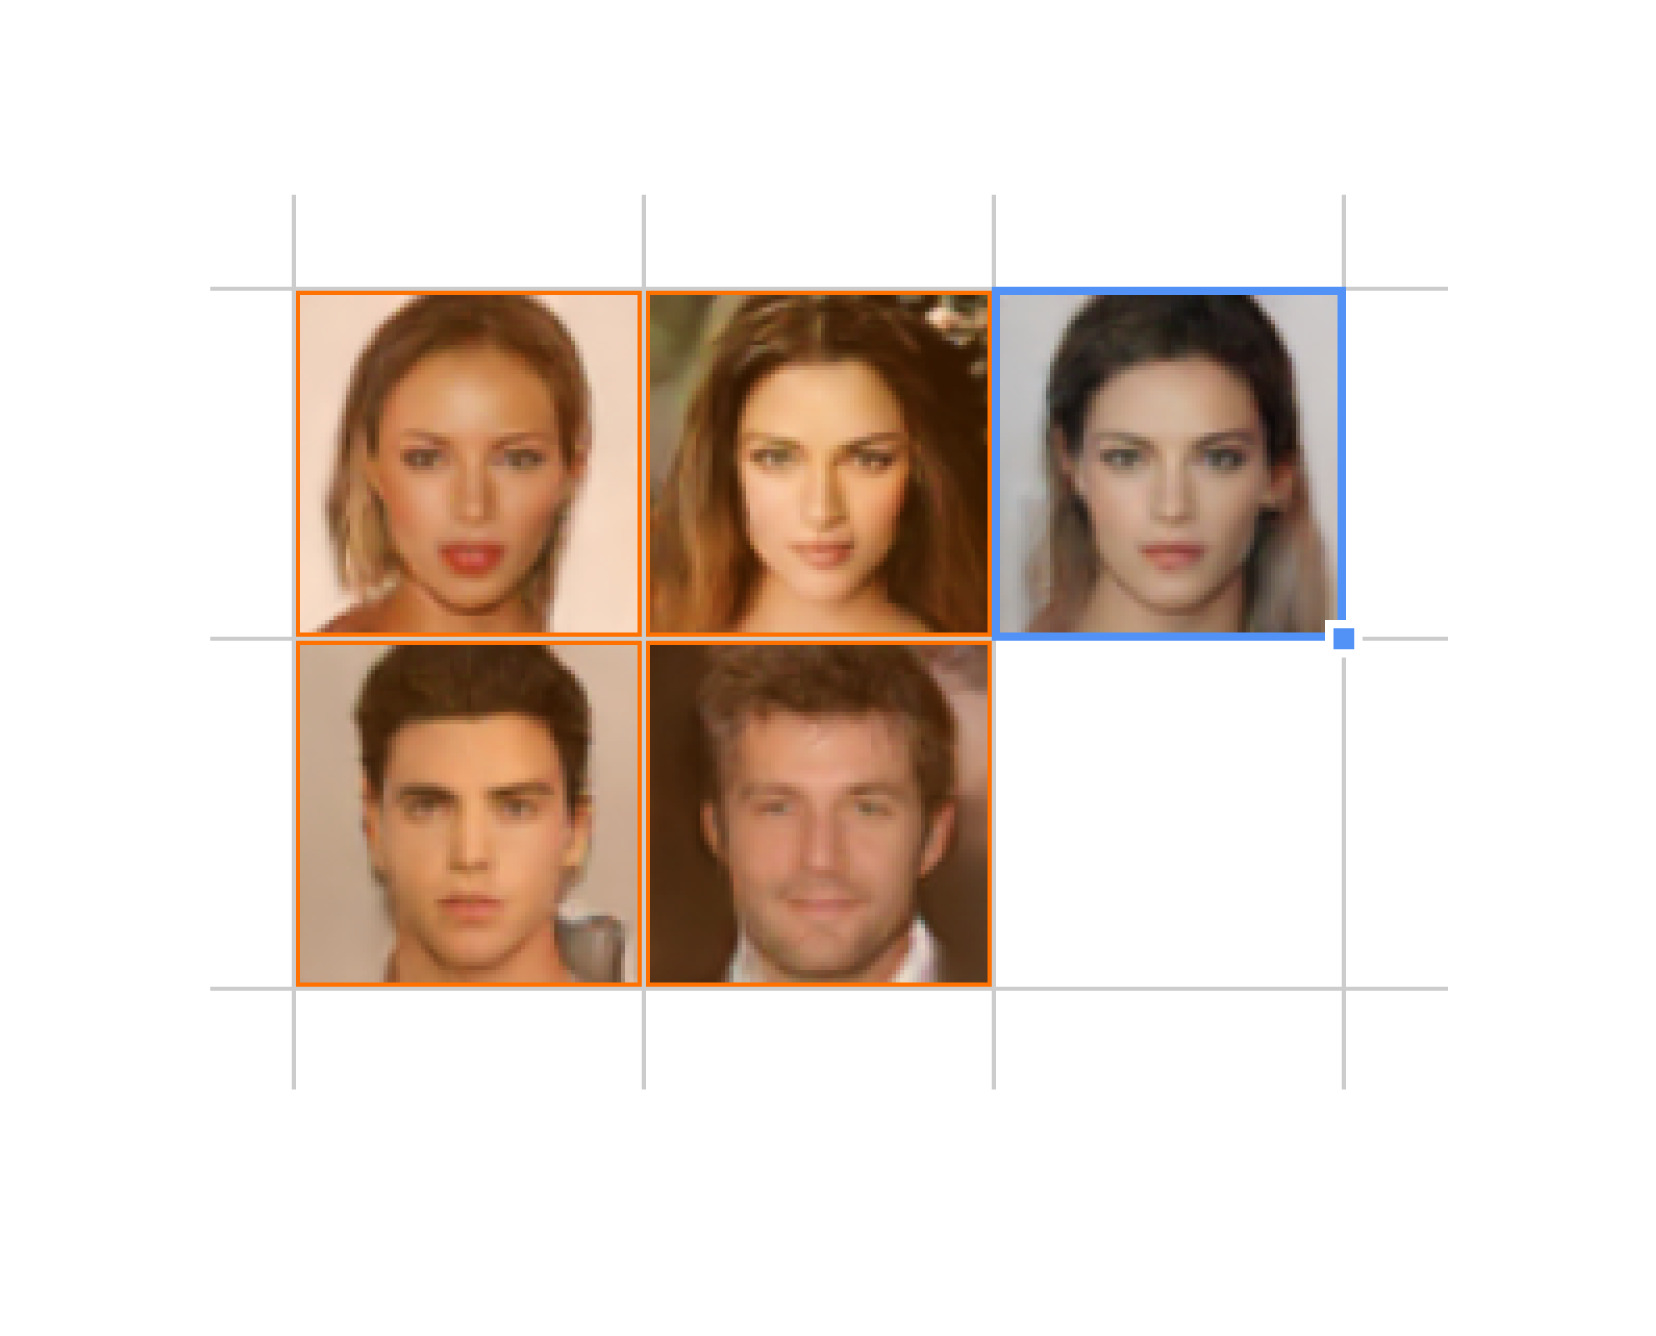
\includegraphics[width=5.5cm]{figs/10-averaging.jpg}
  \caption{Calculating the average reconstruction of a group of latent variables}
\end{figure}

\newpage 
\subsection{Attribute Vectors}
\begin{figure}[ht!]
  \centering
  % \fbox{\rule[-.5cm]{0cm}{4cm} \rule[-.5cm]{4cm}{0cm}}
  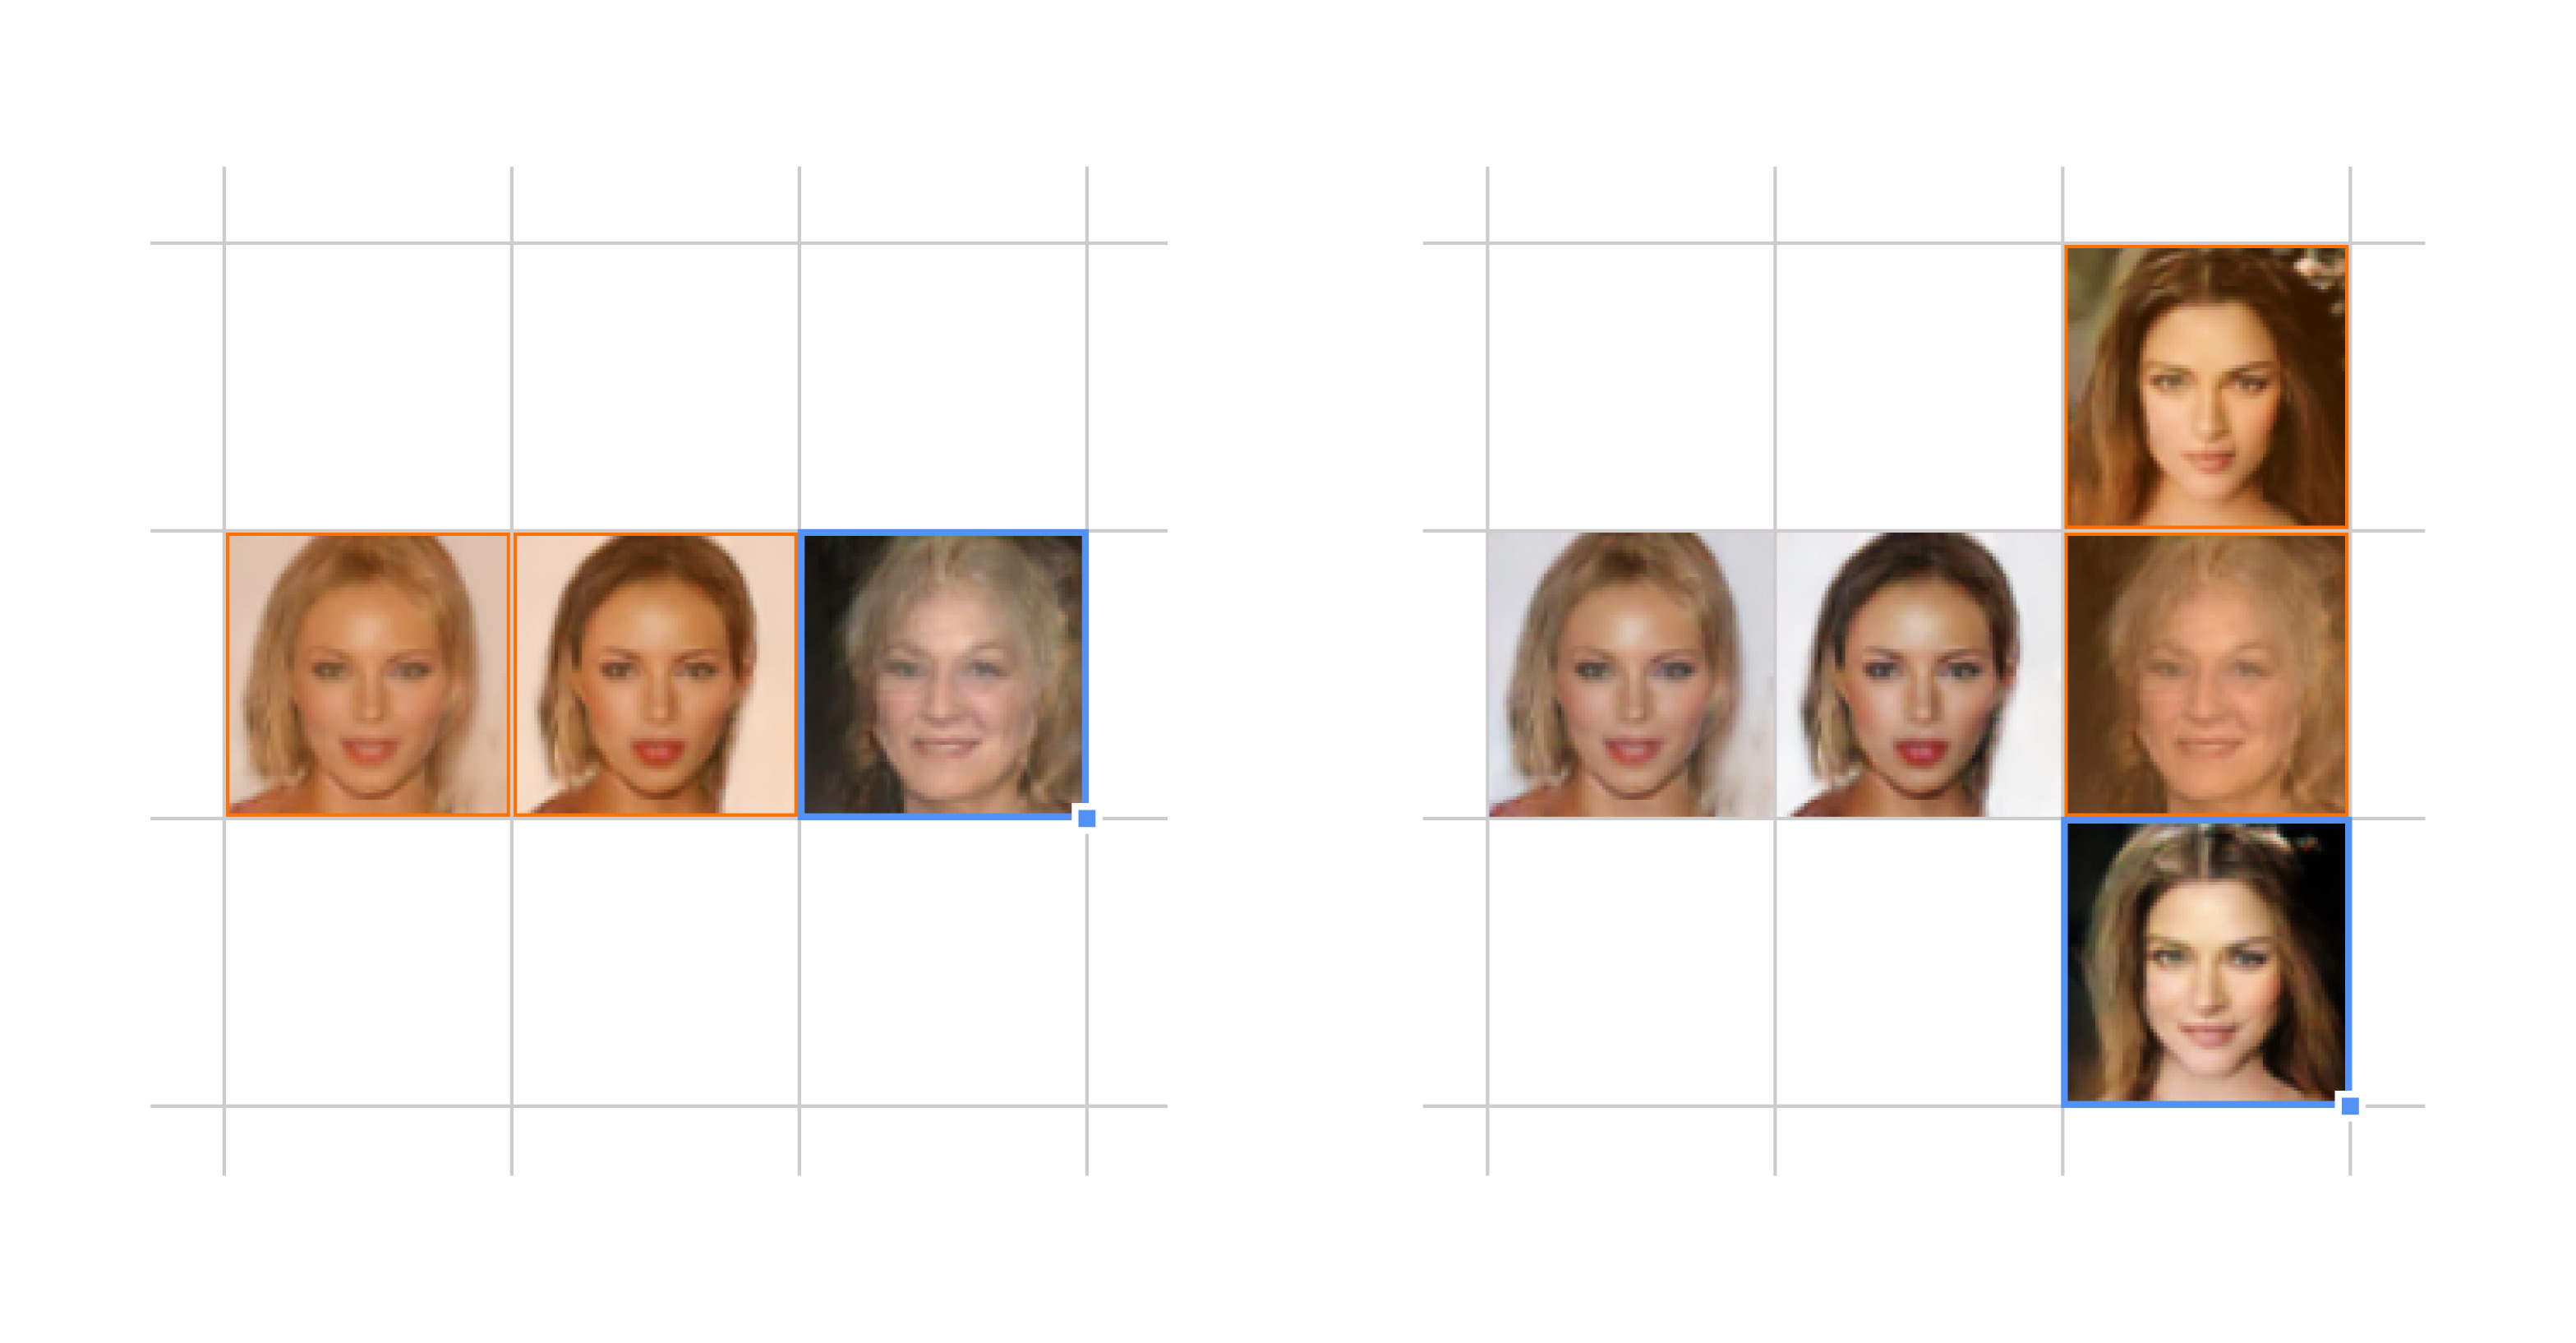
\includegraphics[width=12cm]{figs/09-attribute-vectors.jpg}
  \caption{ Isolating a ‘blonde’ vector by subtraction (left). Adding the attribute vector to a new latent variable (right)}
\end{figure}

Specific attributes can be applied as operations to latent variables. Attribute vectors can be isolated by subtracting a latent vector with desired attributes with one without the attributes. This attribute vector can be added to another latent variable to apply the isolated attribute. The example image shows this two-step process. In the first, a ‘blonde’ attribute vector has been isolated by computing the difference between the highlighted cells. This vector is then applied in the right image by addition. The result is a more blonde version of the initial latent variable.

\subsection{Random Neighbors}
\begin{figure}[ht!]
  \centering
  % \fbox{\rule[-.5cm]{0cm}{4cm} \rule[-.5cm]{4cm}{0cm}}
  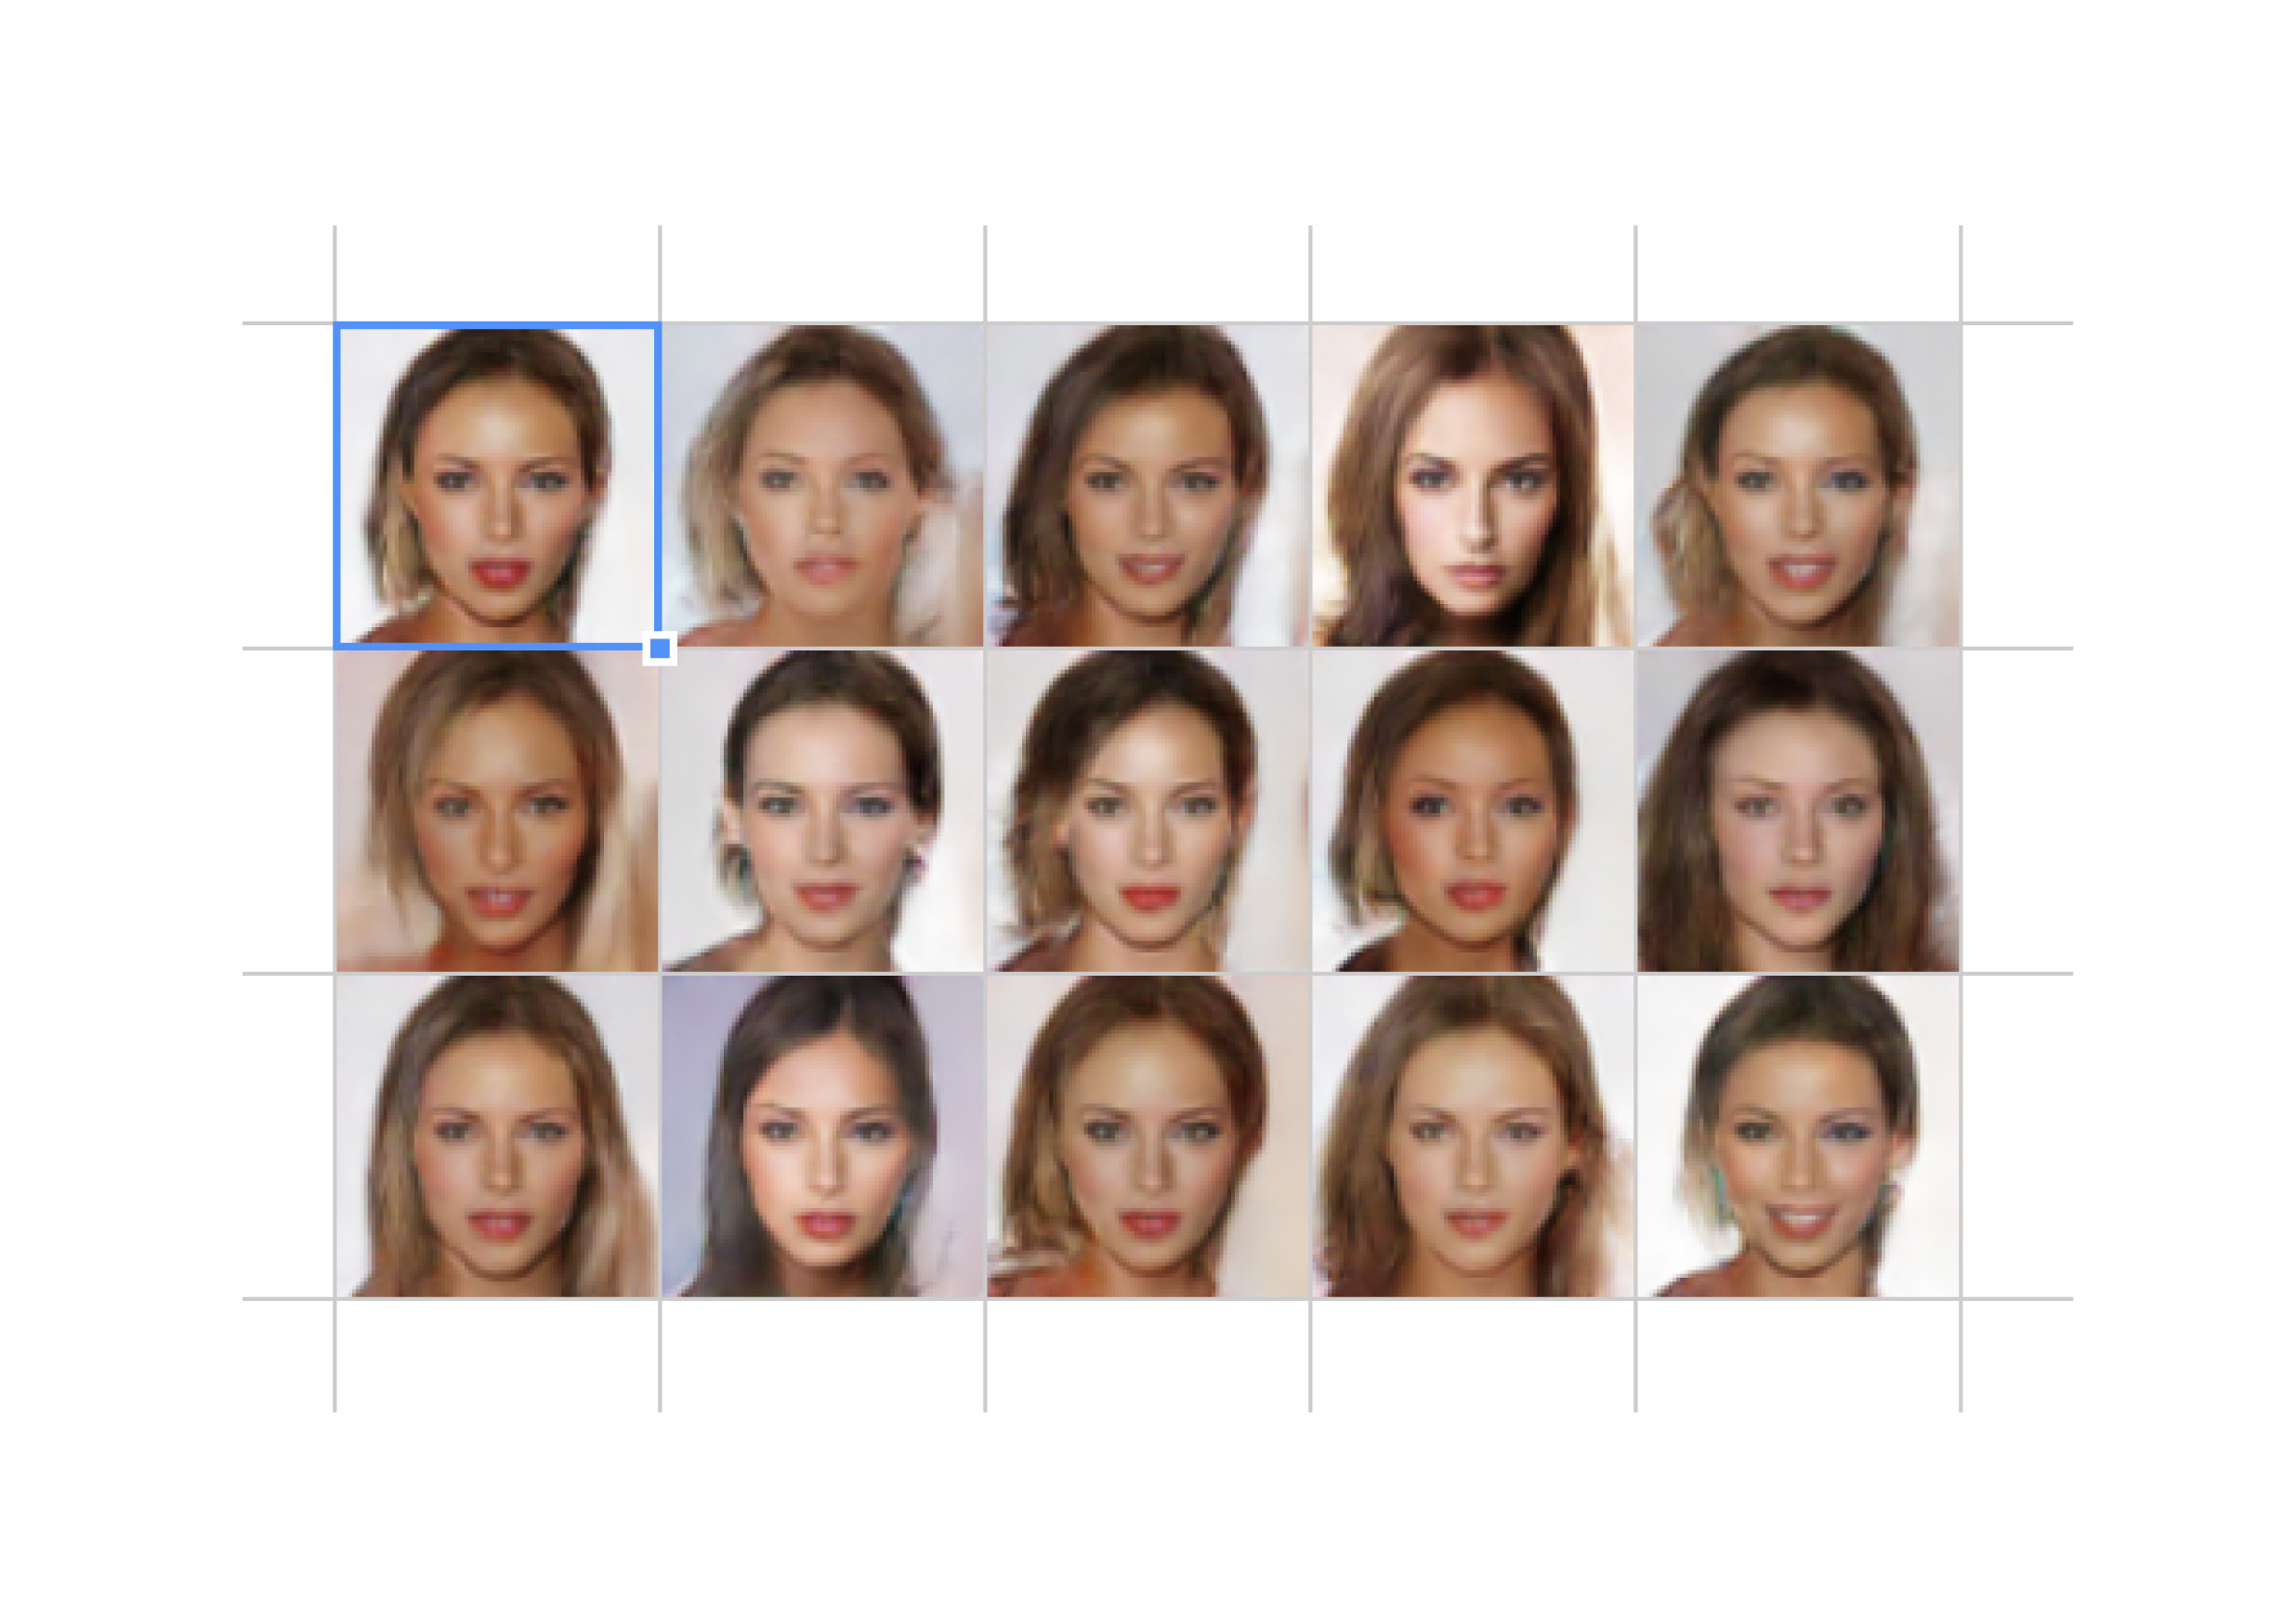
\includegraphics[width=12cm]{figs/11-nearest-neighbours.jpg}
  \caption{A random sampling around the selected cell}
\end{figure}

A random sampling of neighbouring variables can be created using the MOD operation. In the image, the selected cell formed the base from which MOD cells are created.



\end{document}
